%%
%% This is file `mcmthesis-demo.tex',
%% generated with the docstrip utility.
%%
%% The original source files were:
%%
%% mcmthesis.dtx  (with options: `demo')
%%
%% -----------------------------------
%%
%% This is a generated file.
%%
%% Copyright (C)
%%     2010 -- 2015 by Zhaoli Wang
%%     2014 -- 2016 by Liam Huang
%%     2016 -- 2018 by Xuehan Sun
%%
%% This work may be distributed and/or modified under the
%% conditions of the LaTeX Project Public License, either version 1.3
%% of this license or (at your option) any later version.
%%
%% This work has the LPPL maintenance status `maintained'.
%%
%% The Current Maintainer of this work is Xuehan Sun.
%%
\documentclass{mcmthesis}
\mcmsetup{CTeX = false,   
        tcn =1919834 , problem = D,
        sheet = true, titleinsheet = true, keywordsinsheet = true,
        titlepage = true,abstract=true}
\usepackage{palatino}
\usepackage{mwe}
\usepackage{graphicx}
\usepackage{subcaption}
\usepackage{float}
\usepackage{multirow}
\usepackage{indentfirst}
\usepackage{gensymb}
\usepackage[ruled,lined,commentsnumbered]{algorithm2e}
\usepackage{geometry}
\usepackage{caption}
\usepackage{booktabs}
\usepackage{listings}
\usepackage{varwidth}
\usepackage{wrapfig}
\usepackage{caption,subcaption}
\usepackage{amssymb}
\usepackage{bookmark}
\usepackage{breqn}
\geometry{left=2cm,right=2cm,top=2cm,bottom=2cm} 


\newtheorem{assumption}{Assumption}
\begin{document}
\linespread{0.8} 
\setlength{\parskip}{0.5\baselineskip} 
\title{CDSG: Characterization, Derivation, Simulation and Generalization of Extended Floor Field Evacuation Model}
\author{}
\date{\today}
    \begin{abstract}
        The increasing number of terror attacks has aroused growing attention worldwide. As a result, how to  design evacuation plans for different buildings with different gemological layouts has become an urgency.

		We first build \textbf{CDSG}, a novel framework for Characterization, Derivation, Simulation, and Generalization. The \textbf{Extended Floor Field (FF) Model} we derived also cast light on the effictiveness of the evacuation in a certain building. Considering the impact of the geometric layout of a certain building, we apply the \textbf{Grayscale Denoisie Method} to get a matrix from the flat 2-D map of the building. In order to figure out the shortest path to escape, we apply the	\textbf{Hierarchical A* Algorithm} to calculate the \textbf{Static Floor Field} of any given point. Moreover, we develop the \textbf{Extended Floor Field model}, which is based on the \textbf{Floor Field Model}, \textbf{Directional Flow FF Model}, \textbf{Directional Visual Field FF Model}, and \textbf{Remainder Directional Visual Field FF Model}.
		
		To test our Extended FF Model, we apply it to the Louvre Museum and measure the total time steps of the simulation. Then we analyze the sensitivity of the Extended FF Model. Based on the results of our model, we give out certain advice to the supervisor of the Louvre Museum.

		Finally, we generalize our Extended FF Model to meet more requirements and discuss the strengths and weaknesses of our model.
		\begin{keywords}
			Grayscale Denoisie;
			Hierarchical A* Algorithm;
			Floor Field Model;
			Directional Flow FF Model;
			Directional Visual Field FF Model;
			Remainder Directional Visual Field FF Model;
			Cellular Automata
		\end{keywords}

	\end{abstract}

\maketitle


\newpage
\tableofcontents

\newpage
\section{Introduction}
Initially, designers of a building think little of emergency evacuation, because they design architectural structures mainly for presenting beauty and attracting visitors. With emergency accidents occurring one after another around the world such as terror attacks, fire and explosion incidents and earthquake, we find that evacuation plans are urgently needed in many popular destinations. 
Currently, we are contriving of an emergency evacuation model for the Louvre museum leaders to explore a range of options in various circumstances to evacuate visitors from the museum.
The goal of our evacuation plan is to empty the building as quickly and safely as possible, while also allowing the emergency personnel to enter the building as quickly as possible. 
To ensure that individuals leave the building as quickly as possible, we will dynamically design the optimized route from current position of each individual to exits.
To ensure the safety, we will evacuate visitors though the main four entrances: the Pyramid entrance, the Passage Richelieu entrance, the Carrousel du Louvre entrance, and the Portes Des Lions entrance and allow emergency personnel in through some small exit points.

In this work, we propose a framework, named \textbf{CDSG}(Characterization, Derivation, Simulation and Generalization of Extended Floor Field Evacuation Model), which is showned in Figure \ref{frame}: 
\begin{figure}[H]
    \centering
    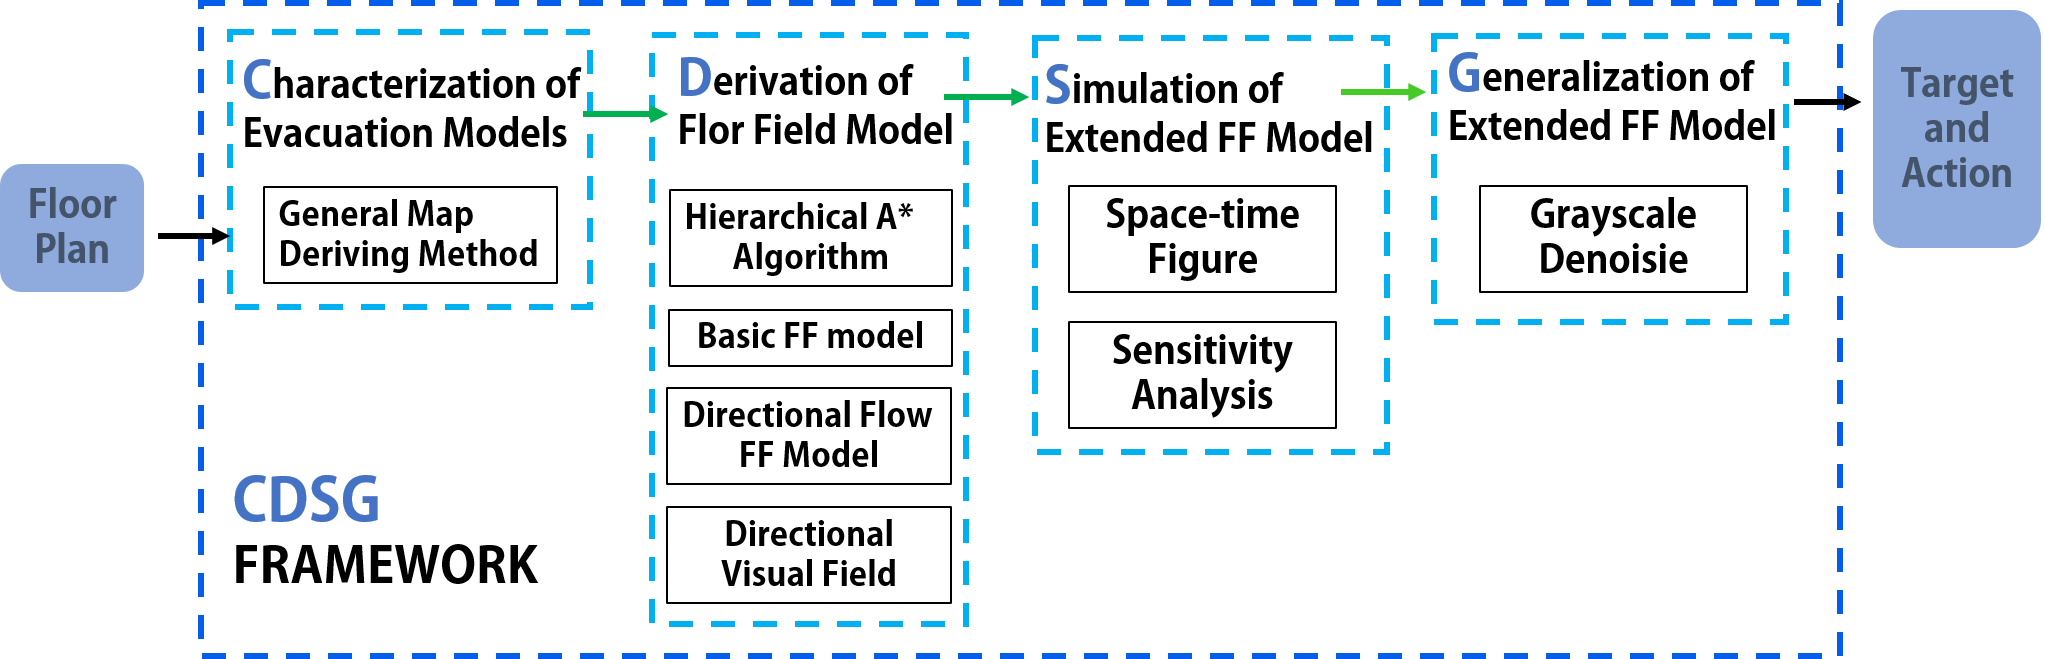
\includegraphics[width=0.9\textwidth]{framework.png}
    \caption{Framework of CDSG}
    \label{frame}
\end{figure}


\section{Assuptions}
\begin{assumption}
    The diversity of visitors will not have great influence on the effectiveness of the evacuation.
    \end{assumption}
    Our team treat all the visitors alike. That is to say:
    \begin{itemize}
    \item The language that each visitor speaks does not have direct impact on their choice of route to leave the building. 
    \item The speed the visitors move are the same.
    \item Without arrangement, the visitors will use the same strategy to choose the route.
    \end{itemize}
    \begin{assumption}
    Only emergency personnel and museum officials will get through the available exit points to enter the building.
    \end{assumption}

    Those secret points are not well-known by the public and our team cannot figure out the position of those points. It is reasonable to assume that ordinary visitors will not choose those gates to escape the building since they do not even know the existence of those exit points and the safety of those point are not guaranteed. Consequently, we will not utilize any of those exit points as additional exits.
    \begin{assumption}
    The Interactive Floor Plans given on the official site of the Louvre Museum can correctly show the passage and relative size of each gallery in the museum.
    \end{assumption}
    Our team use the Interactive Floor Plans to establish our model, so the accuracy of the information given on that plan contributes the accuracy of the result of our model.
    

\section{Abbreviations and Definitions}
Main symbols used in the following model are shown in the Table1.
\renewcommand\arraystretch{1.4}

\begin{figure}[H]
\captionsetup{type=table}
\captionsetup{font=small, labelfont=bf}
\caption{Main Symbols Used in the Following Model}
\begin{tabular}{cp{35em}}

\toprule
Symbol &Meaning \\
\midrule
$P_{ij}$& the possibility of a transferring from the central cell to cell$(i, j) $ \\
\hline
$P_{ij}^{rX}$& the possibility of cell $(i, j)$with $ r$ as the radius of its visual range  transferring to its neighoring cell in the direction $X$.\\
\hline
$S_{ij} $& Static Floor Field of cell$(i, j)$: describing the effect of  geometric layout on evacuation \\
\hline
$D_{ij}$ & Dynamic Floor Field of cell $(i, j)$:representing virtual trajectory left behind by individual movement\\
\hline
$V_{ij}^{rX} $& The number of the cells in the Direction Visual Field with direction X and radius r of cell $(i, j)$
\\
\hline
$RV_{ij}^{rX}$ & The number of the empty cells in the Remainder Direction Visual Field with direction X and radius r of cell $(i, j)$
\\
\hline
$O_{ij}^{rX} $&The number of the cells that are occupied by a visitor in its influenced area in the X direction\\
\hline
$C_l^m$&efficacious spare capacity of the entrance $m$\\
\hline
$k_S$ & sensitive parameter of Static Floor Field :reflecting visitors' familiarity with interior structure of a room\\
\hline
$k_D$ &sensitive parameter of Dynamic Floor Field: reflecting the trend of an individual following others\\
\hline
$k_V$ & sensitive parameter of $V_{ij}^{rX}$
\\
\hline
$k_{RV}$ &sensitive parameter of $RV_{ij}^{rX}$
\\
\hline
$k_{O}$ &sensitive parameter of $O_{ij}^{rX} $
\\
\hline
$k_{C}$ &sensitive parameter of $C_l^m$
\\
\hline
$N$ & normalization factor\\
\hline
$\mu_{ij}$& reflecting whether the cell$(i, j)$ is occupied by other visitor\\
\hline
$\xi_{ij}$&reflecting whether the cell$(i, j) $ is occupied by obstacle\\
\hline 
$E_{ij}$& the distance from cell $(i, j)$ to the nearest exit\\
\hline
$Sij$& the $j^{th}$ stair on the $i^{th}$ floor\\
\hline
$Eij$& the $j^{th}$ exit on the $i^{th}$ floor\\
\hline
$\alpha$&the diffusion coefficient\\
\hline
$\beta$&attenuation coefficient\\
\hline
\bottomrule
\end{tabular}

\end{figure}


\section{Characterization of the Evacuation Model}
\subsection{Choice of The Model}
With the development of economy and society, the population in modern city and the density of people in public areas are both increasing. Consequently, various models simulating 
evacuation were devised and improved, which can be divided into macro model, micro continuous model, and micro discrete model.

Fruin first put forward the macro model. The macro model think of the crowd as a whole, and it contains two types of models: Fluid Dynamics model and Network Node Model. The Fluid Dynamics Model regards the movement of crowd as fluid. The Network Node Model describes the rooms with nodes and portray the stairs, elevators, and doors with edges. However, in this model, we will lose the spatial information such as size, internal structure, and shape of rooms, in the process of abstracting. Moreover, both models neglect personal psychological factors and interaction between individuals.

Micro continuous model includes Physical Model and Control Model. Typical examples of Physical Model are Magnetic Force Model raised mainly by Okazaki \cite{97} and Social Force Model raised mainly by Helbing. Adopting the Law of Coulomb, the Magnetic Force Model describes the pedestrians as objects in magnetic field, every pedestrians and obstacles as positive poles, and destinations as negative poles. Pedestrians decide their direction and speed of moving according to magnetic force and force which is used to avoid collision. However, because the magnetic field intensity is arbitrarily given, it is impossible to test and verify it with reality. In the Social Force Model, we show various intrinsic driving factors of pedestrians with physical forces and uses the traditional vector summation method to calculate the linear effects of various intrinsic driving factors on pedestrians. Finally, we use resultant vector to represent comprehensive effect of different factors, thus making pedestrians move like particles under the Newton’s Second Law. However, as human’s consideration of external factors is obviously non-linear, we cannot express the real situation using this model. Moreover, because the synthetic action may not be compatible with single action, conflict between human and obstacles may happen. 

The most commonly used model of micro discrete type is CA Model (The Cellular Automata Model) . \cite{92} Von Neumann and Stanislaw Ulam first successively put forward the basic thought of CA Model. After careful comparison, we find that traditional CA model with modifications can be used in this problem.

In CA, we discretize space into equal cells with regular shape. Each cell contains the state information of the cell. In principle, the possible state of a cell is limited and discrete. Then we build a series of rules to construct the model. We determine the state of a cell at the next moment by the current state of the cell and the current state of its neighborhood. With multiple iterations, we can simulate the change of complex objects. In real evacuation circumstances, the action of an individual depends on the status of the individual itself and the surrounding crowd, which is similar to the rules of CA. \cite{32} \cite{60} To make a CA model, we should first work on discretization and decide attributes.

\subsection{Basic Settings}
In our CA models, we discretize evacuation space into two-dimensional cells. Each cell has three basic state: empty, occupied by one obstacle or occupied by an individual. 

\begin{itemize}
\item  size of a cell 

The average width of an individual is approximately 50cm. As every cell can be occupied by an individual, the length of the cell should be the same as the average width. To simplify the
calculation, we use
\begin{equation*}
1\ cell= 50\ cm
\end{equation*}
\item  time unit

To ensure that the movement of an individual is reflected at an appropriate speed, we determine the time unit as size of cell divided by normal speed of pedestrians. According to Bohannon, Richard W and Andrews, and A Williams’s work, normal walking speed is 0.51-1.27 miles per second. To simplify our model, we see walking speed as 1mile per second. We expect that in one turn of our CA model, an individual makes one action. Consequently, we decide 
\begin{equation*} 
	1\ time\ unit = 0.5\ s
\end{equation*}
\end{itemize}


\subsection{Map Deriving}
In preparation for our model, we process maps of Louvre.\cite{} Take map of floor 0 as an example. We first omit redundant information indicated in the map and traverse every pixels in the tourist map shown in Figure 2. 

\begin{figure}[H]
\parbox[b]{.5\textwidth}{
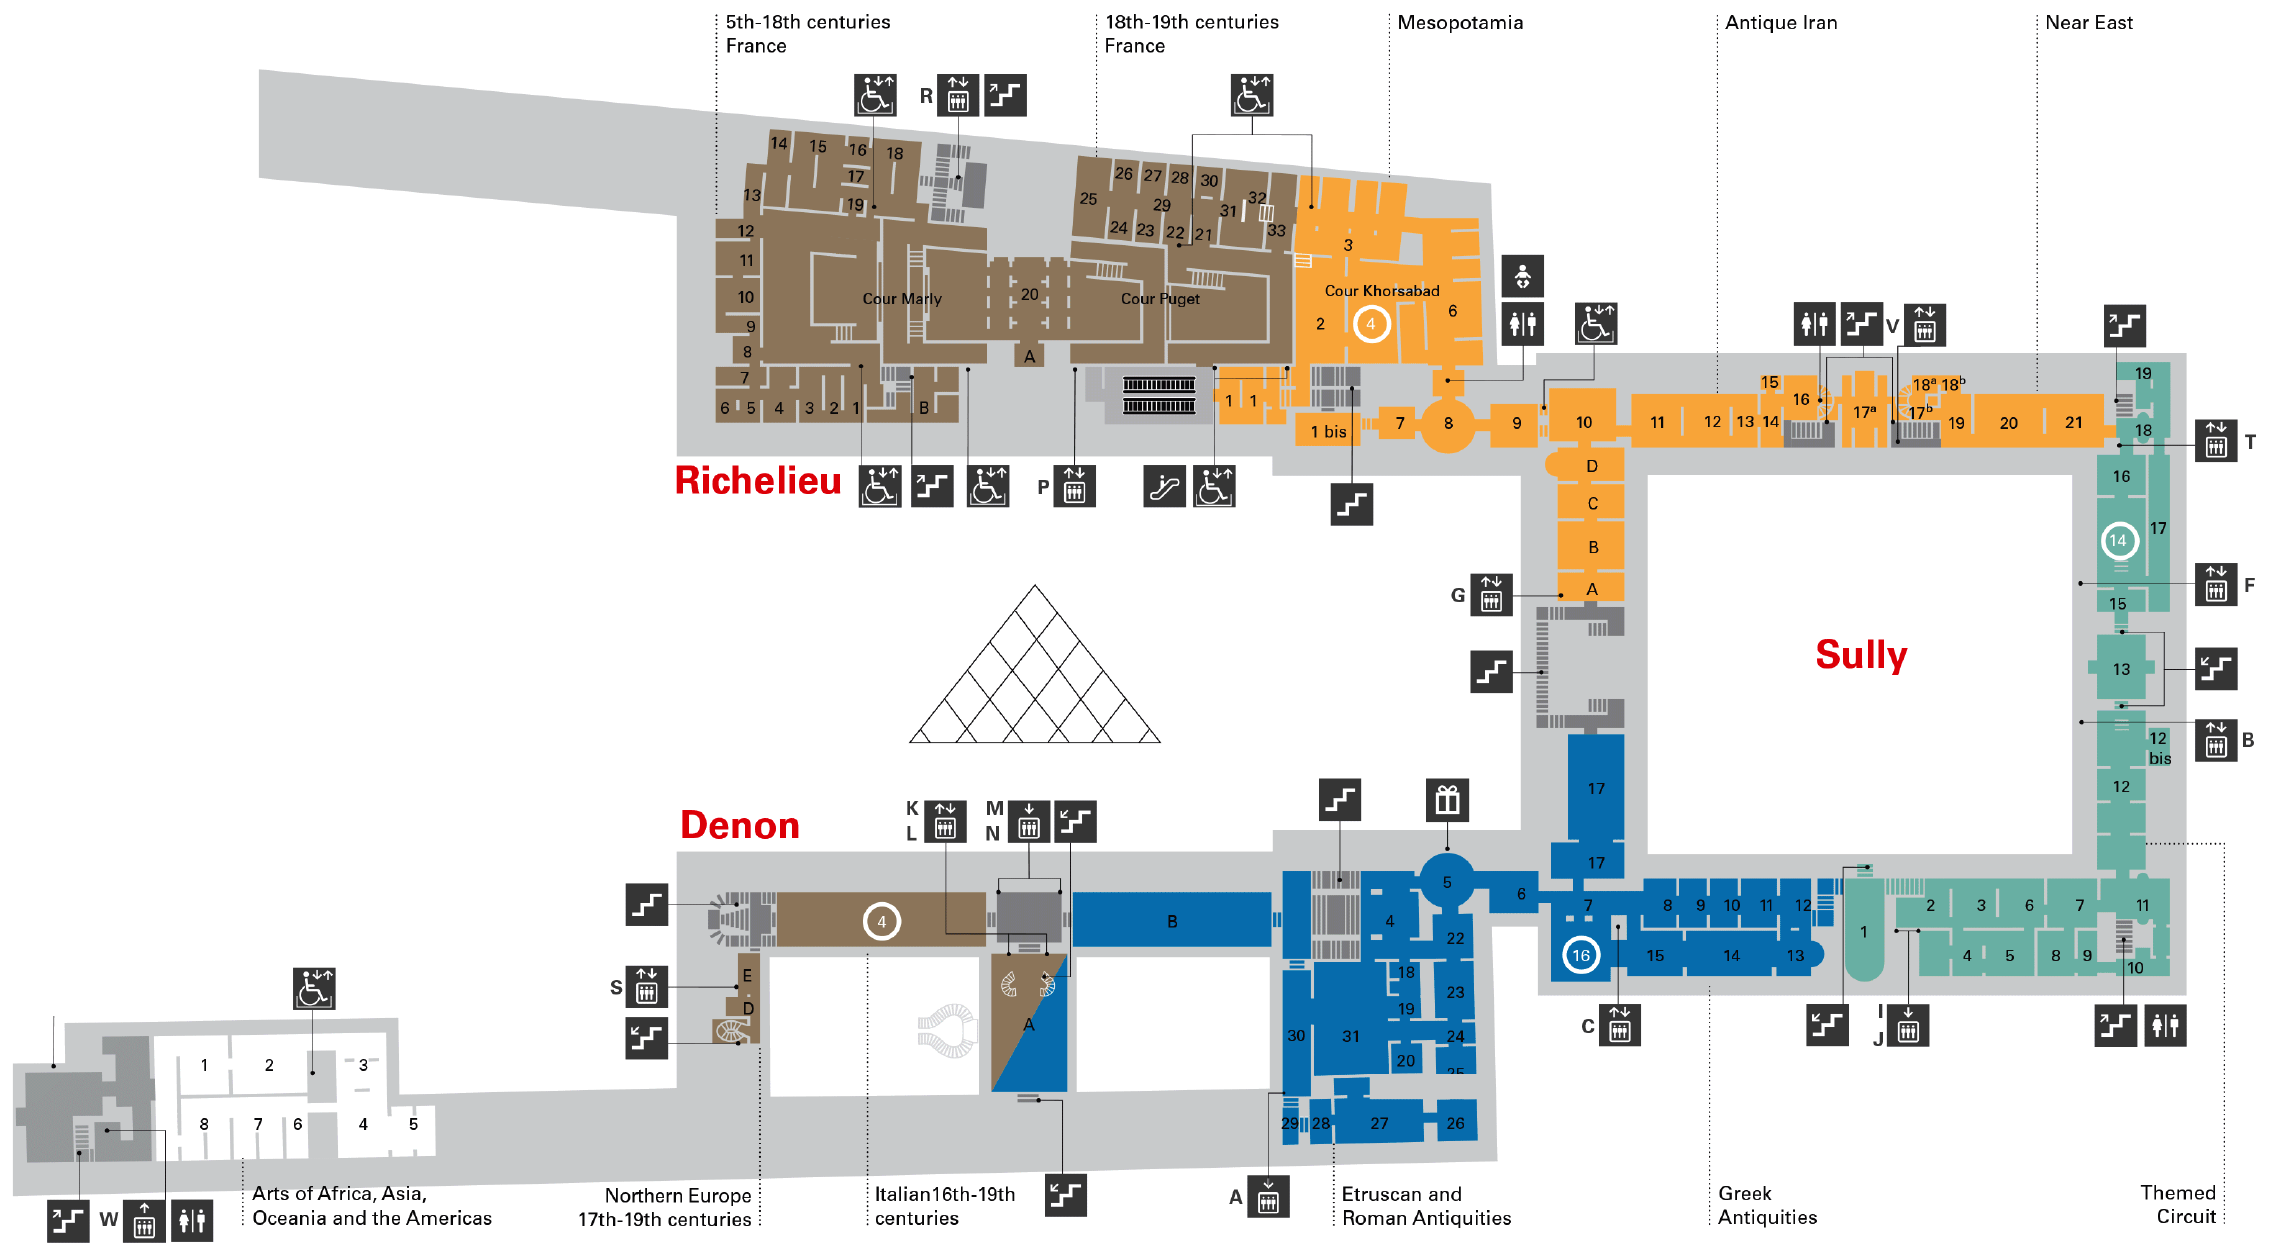
\includegraphics[scale=0.25]{floor0_photo}
\centering\captionsetup{font=small, labelfont=bf}\caption{Original Guide  Map of Louvre}
}
\parbox[b]{.5\textwidth}{
\includegraphics[scale=0.12]{floor0_bw}
\centering\captionsetup{font=small, labelfont=bf}\caption{Color Processed  Map}
}
\parbox[b]{.5\textwidth}{
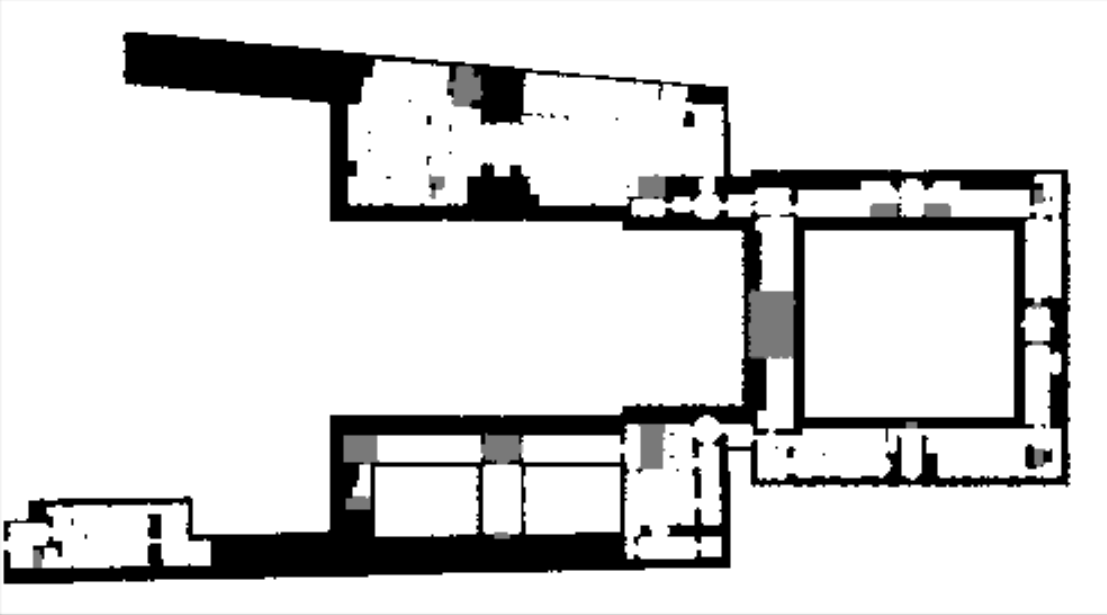
\includegraphics[scale=0.24]{floor0_noise_pre}
\centering\captionsetup{font=small, labelfont=bf}\caption{Denoised Map}
}
\parbox[b]{.5\textwidth}{
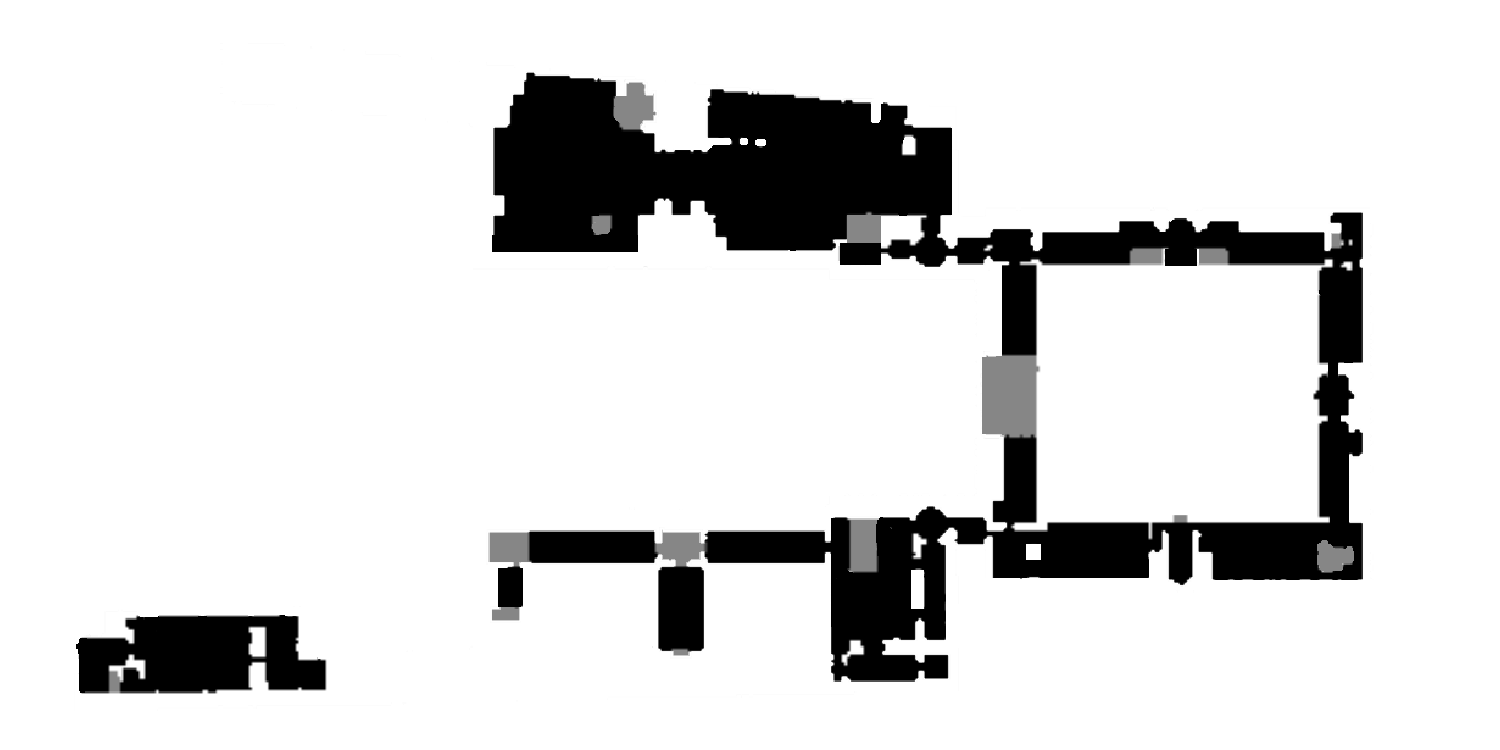
\includegraphics[scale=0.47]{floor0}
\centering\captionsetup{font=small, labelfont=bf}\caption{Final Analogous Map}
}
\end{figure}

We change the RGB value of each pixel to an appropriate value. If the initial color of an pixel is light gray, we change its RGB value to (0, 0, 0). If the initial color of an pixel is dark gray, we change its RGB value to (1, 0, 0). We change the RGB value of rest pixels to (255, 255, 255). the Python Program of this process is attached to our essay in Appendix. Then we have black representing obstacles such as walls, gray representing elevators and stairs, and white filling other area. Now we get black-white-gray map shown in Figure 3. 

However, there exists a large number of hot pixel (random black dots caused by interference on image signals) in the picture. There are four method of denoising: Median Filtering or Mean Filtering of salt and pepper noise as well as that of Gause noise. Their processing result are shown in Figure 6. 

\begin{figure}[H]
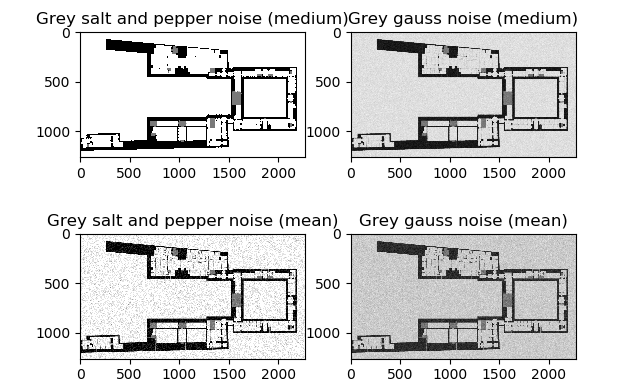
\includegraphics[scale=0.9]{model_comparision},
\centering\captionsetup{font=small, labelfont=bf}\caption{Processing Method Comparision}
\end{figure}


Obviously, the Median Filter of Salt and Pepper Noise works best. Consequently, we use this method to denoise. The Median Filtering is an typical non-linear technique. Usually, the gray value of impulse interference is largely different from image signal. The basic idea of Median Filtering is to replace one gray value of a pixel with the median of its neighborhood gray value so that the gray value of this pixel cannot be influenced by extreme value and get close to the real value. For example, for a pixel$(i, j)$ ’s neighboring  $3\times 3$ area, we obtain gray value of each pixel in this area first and put them in an aggregate $ A_{ij}$ .This area is shown in Figure 5. 


Then we put the values of $A_{ij}$ in numerical order. Finally, we decide this pixel's value on the fifth value. 

After Median Filtering repeatedly, we can denoise and reserve fringe detail of image at the same time. The processing result is shown in Figure 4. Besides, the Python program of denoising is attached to out essay in Appendix B. 

Then we develop an algorithm to change color of the map and regularize the edge of shapes by extracting boundary where gray value of pixels changes sharply then arranging the pixels on the boundary neatly. The final image we get are shown in Figure 4. Moreover, the processed maps of other three floors are shown in Figure 7.

\begin{figure}[H]

\parbox[b]{.35\textwidth}{\centering
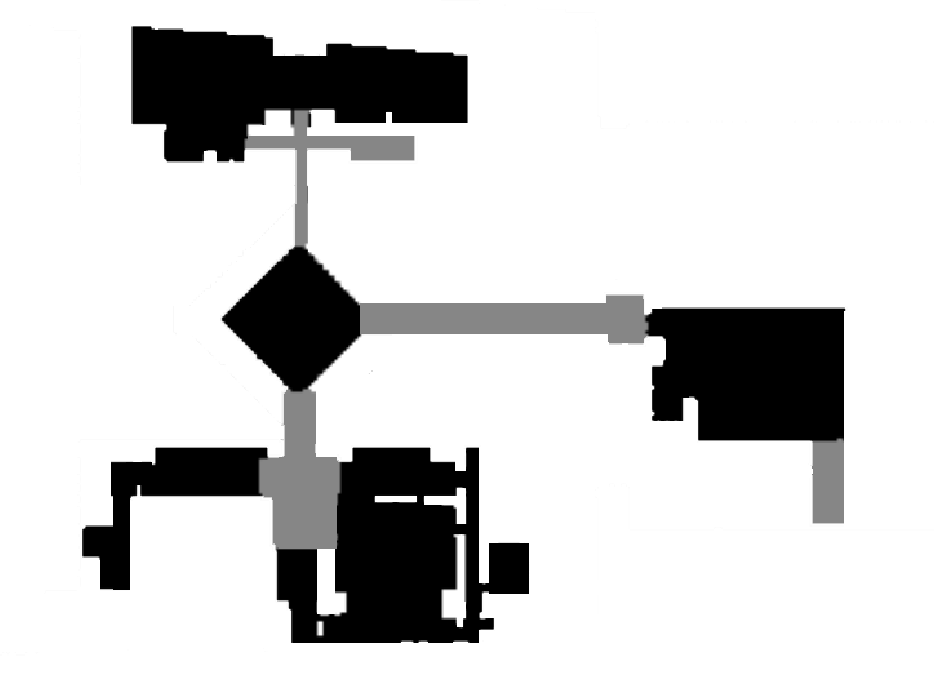
\includegraphics[scale=0.45]{floor-1}
\subcaption{Floor -1}}
\parbox[b]{.3\textwidth}{\centering
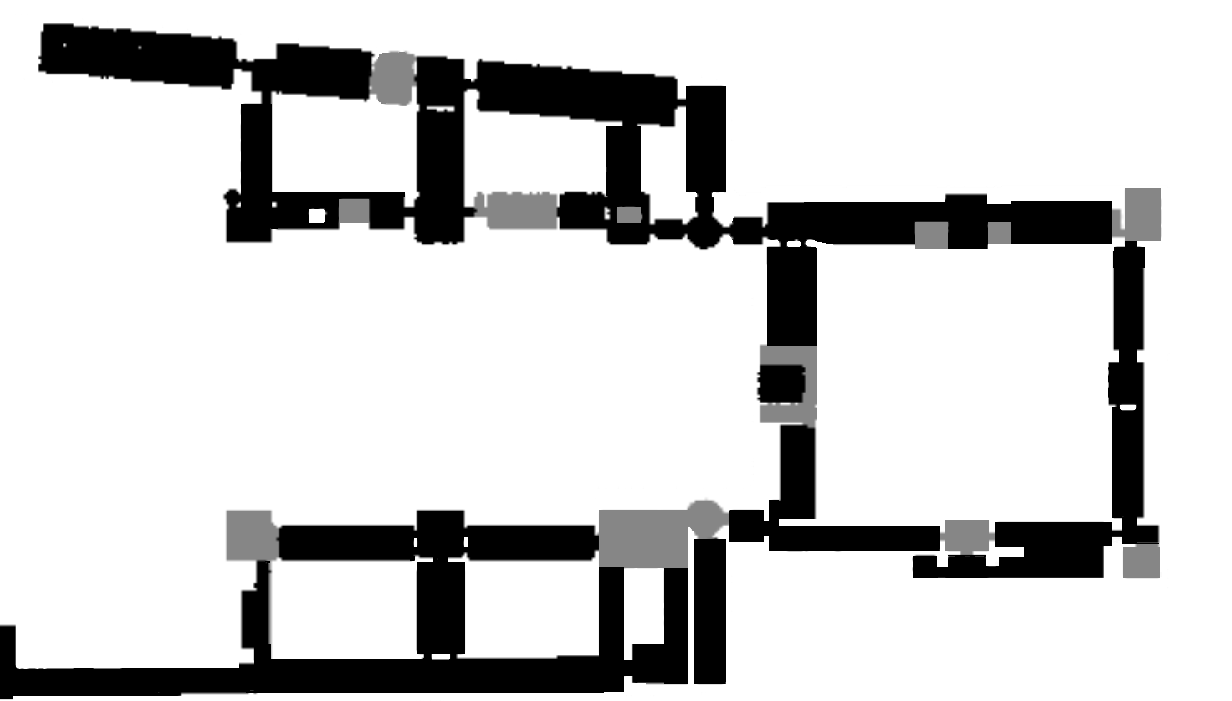
\includegraphics[scale=0.4]{floor1}
\subcaption{Floor 1}}
\parbox[b]{.3\textwidth}{\centering
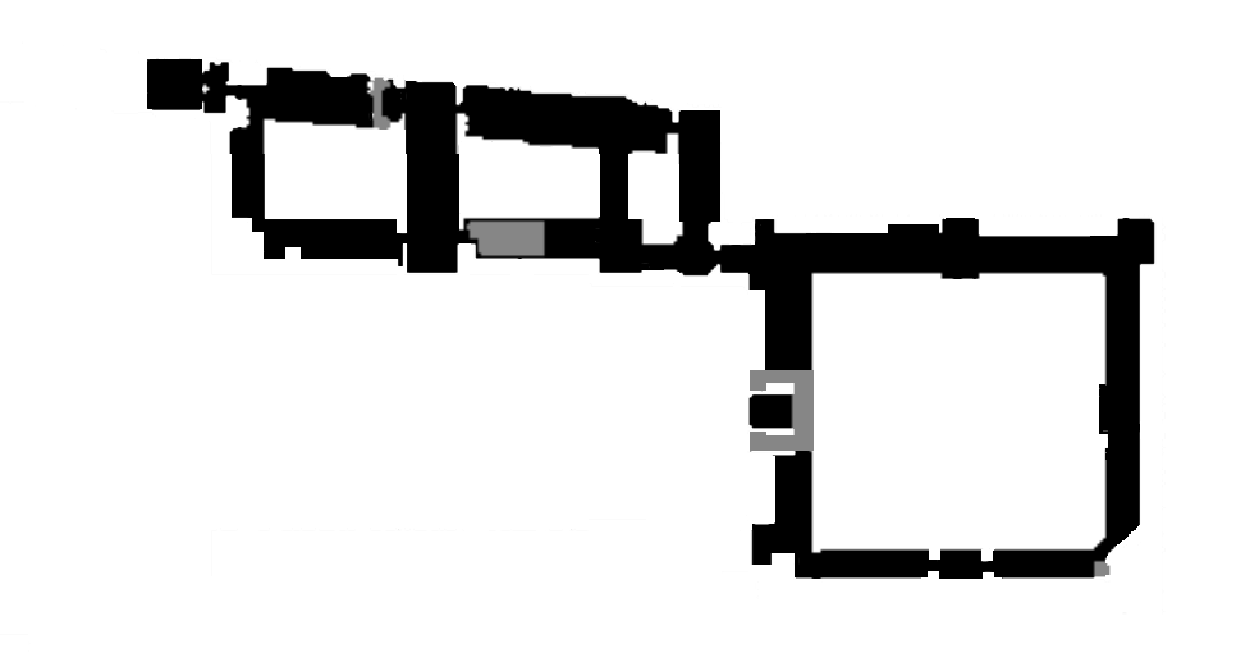
\includegraphics[scale=0.45]{floor2}
\subcaption{Floor 2}}
\caption{ Processed Map of Other Three Floors}
\end{figure}




\section{Derivation of Floor Field Model}
\subsection{Hierarchical A* Algorithm}
    We first use A* algorithm to find the Shortest route in each floor map. A* algorithm performs well on finding the shortest path. Different from Dijkstra and Floyd algorithm, A* combines the advantage of Breadth First Search and Dijkstra algorithm: While heuristic search improves the efficiency of the algorithm, it can ensure to find an optimal path. The pathfinding process can be completed in the following 3 steps, as is shown in Figure \ref{A_star}:

    After the pathfinding process, we acquire an open list. Then  we need to choise the next step. The fomula is shown in Equation \eqref{bla}:
    \begin{equation}
        f(n) = g(n) + h(n)
    \label{bla}
    \end{equation}

    \begin{figure}[H]
        \centering
        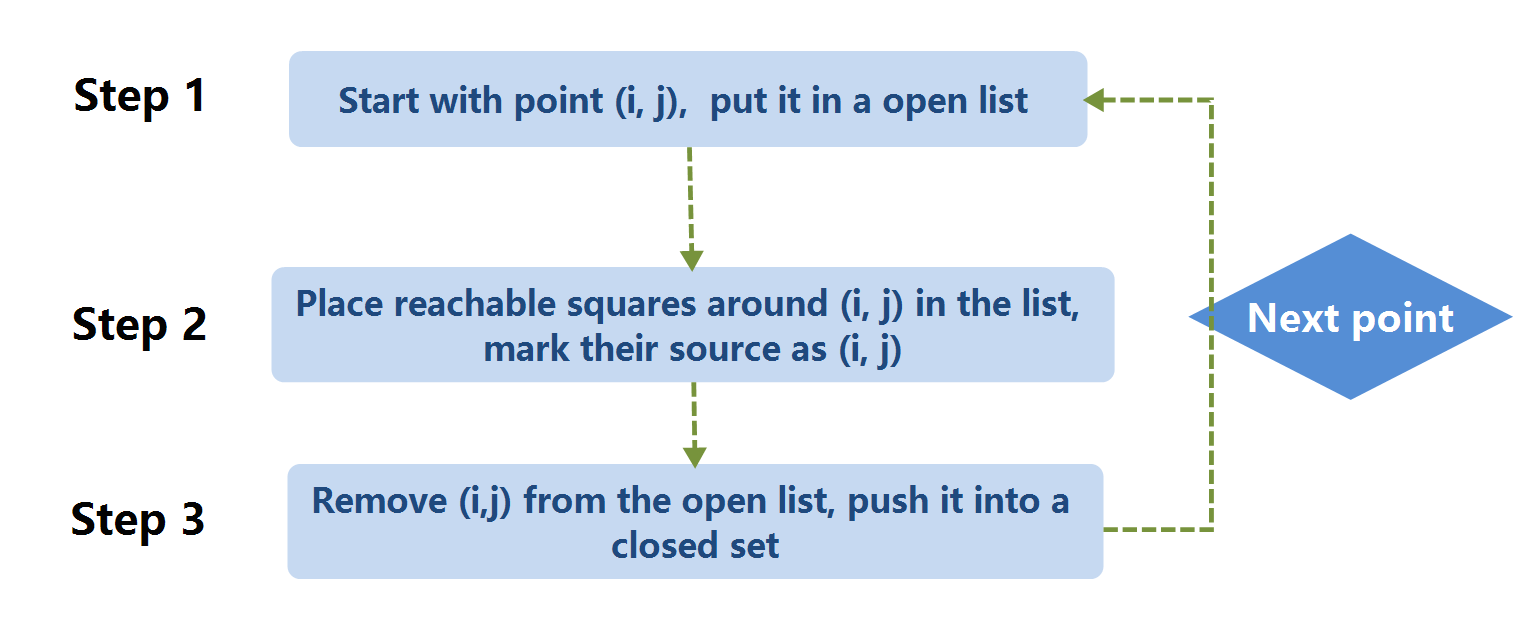
\includegraphics[width=0.75\textwidth]{A_star.png}
        \caption{A* Algorithm Pathfinding Process}
        \label{A_star}
    \end{figure}


    $h_n$ indicates the the distance from staring square to current square, and $h_n$ indicates the distance from the upcoming square to the destination square. The sum of the two values means the possible path of current estimation, and the square with the  smallest value is the next moving square. Then, we repeat the aboving steps, until the destination square is in the neighboring square. 

    After calulating the shortest route in each floor and storing them in .csv format, we come closer to the data $S_{ij}$ in all floors. The problem can be converted into a Traversal of Tree problem, and we choose a point in the $2_nd$  floor as the example, as is shown in Figure \ref{tree}:
    \begin{figure}[H]
        \centering
        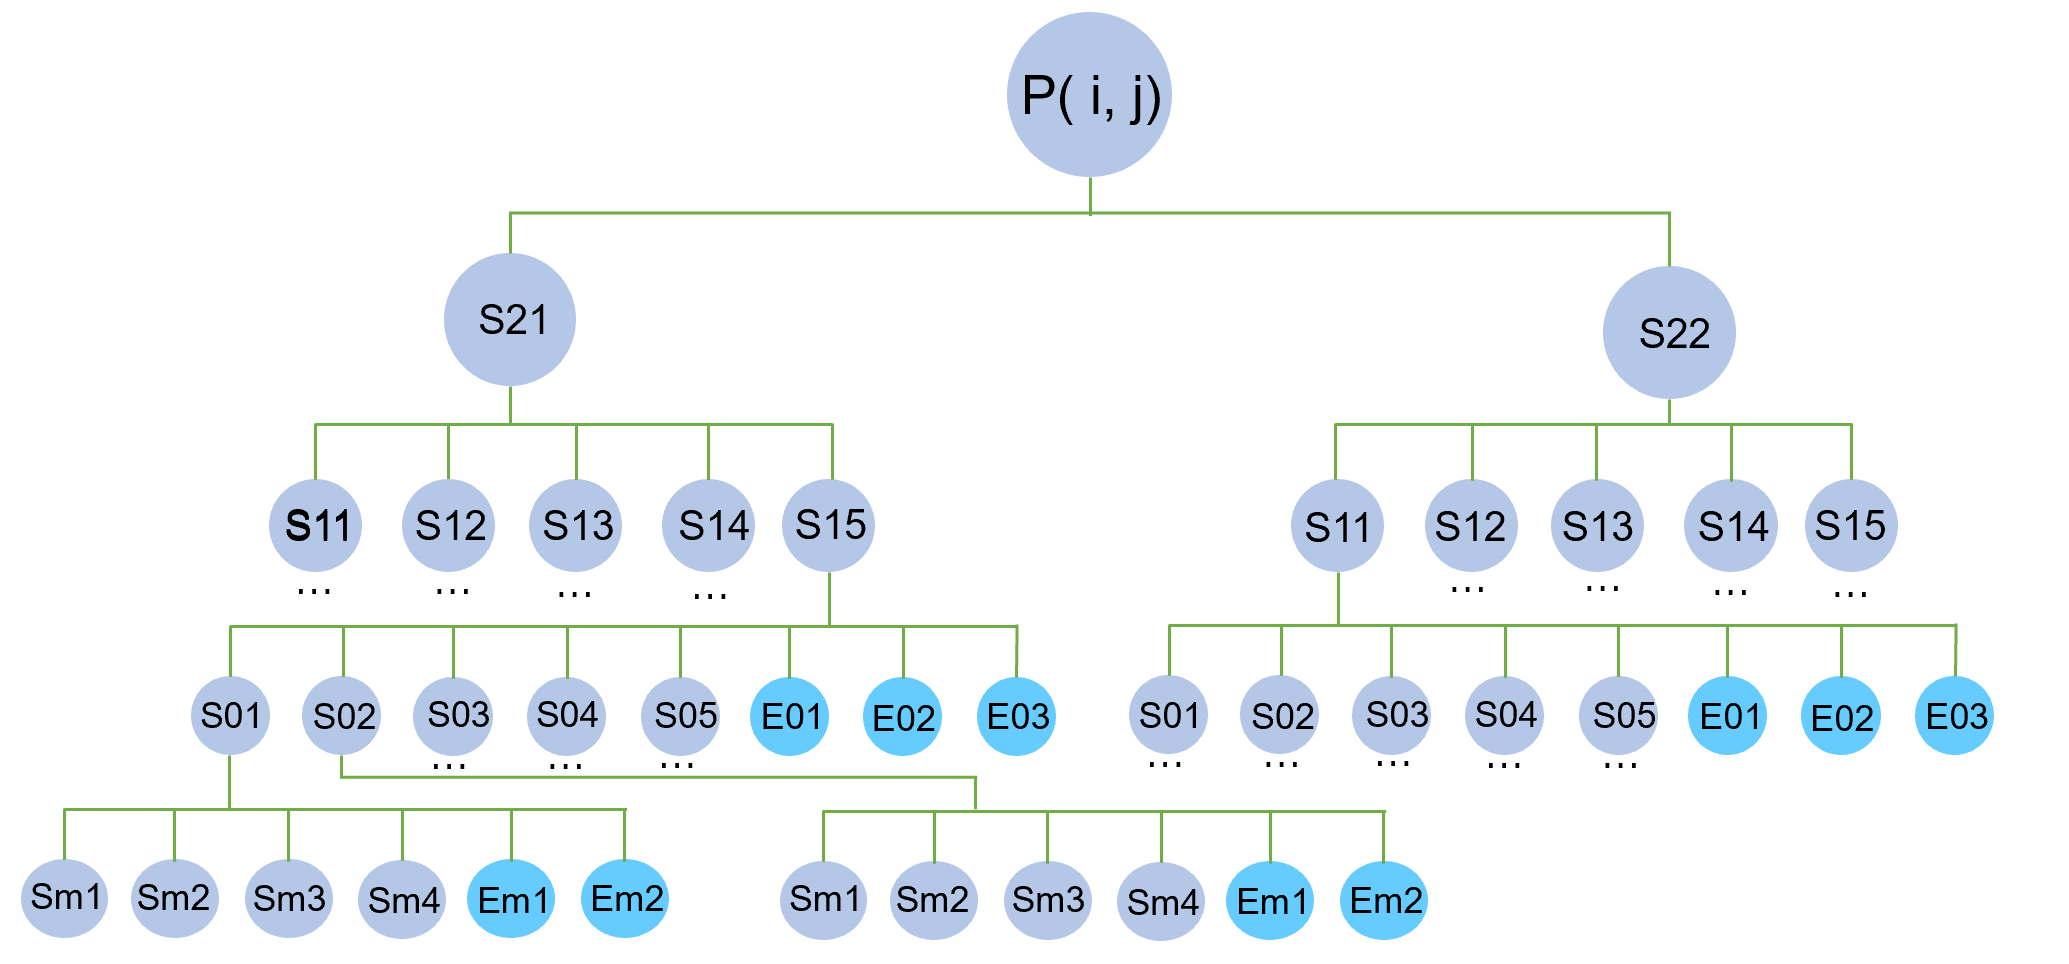
\includegraphics[width=0.95\textwidth]{tree.png}
        \caption{Traversal of Tree}
        \label{tree}
    \end{figure}

    $P_{ij}$ is a point on the $2_{nd}$ floor, Sij means the $j^{th}$ stair on the $i^{th}$ floor, and Eij means the $j^{th}$ exit on the $i^{th}$ floor(m means -1). After the tree is  traversed for N times, we get the data of $S_{n_{ij}}$, which means the shortest path from the point in pixel(i, j) to all exits. N is calculated in Equation \eqref{N}, and $S_{n_{ij}}$ is given by Equation \eqref{Snij}:
    \begin{equation}
        N = n_{floor2} \times n_{floor1} \times [n_{exit0} + (n_{floor0} \times n_{exitm1} ) ] = 130 \quad times
    \label{N}
    \end{equation}
    \begin{equation}
        S_{ij} = \min\limits_{n_E} \{S_{P_{(i,j)}}+ {\sum\limits_{t = 1}^{T-2} S_{S_{kl}}}  + S_{E_{mn}} \}
    \label{Snij}
    \end{equation}

    In Equation \eqref{Snij} T is the traversal times, $S_{S_{kl}}$ is the $l^{th}$ stair on the $k^{th}$ floor, $S_{E_{mn}}$ is the $n^{th}$ door on the $m^{th}$ floor, and $n_e$ is the total number of exits.

\subsection{Basic FF model}
Inspired by the movement of animals, Kirchner \cite{65} established an evacuation model to characterize the interaction between different visitors. The evacuation space is discreted into cells. Each cell only has three status: empty, occupied by a visitor, or occupied by an obstacle. Time is also descreted into time steps. Each time step, a visitor can move to its adjacent empty cell according to a certain transition probability. Visitors may also remain in their original cell. The transition probability is defined by the \textbf{Floor Field} of each cell. Physically, the higher the floor field of a cell is, the more appealing it is to the visitors nearby. Transferring large-scale and long-distance effects into local effects is our main purpose of introducing Floor Field into our model. Like Cellular Automata model, \textbf{Floor Field Model} is simple and effictive. 

We use Floor Field to decide transition possibility, show how attractive a cell is to an individual, and then show both static and dynamic attributes of cells. The Floor Field can be devided into 2 categories: Static Floor Field and Dynamic Floor Field. The probability of the transition is defined in Equation \eqref{basic}.

\begin{equation}
	P^U_{ij}=N_{ij}\cdot e^{\left(k_SS_{i-1,j}+k_DD_{i-1,j}\right)}\left(1-\mu_{i-1,j}\right)\xi_{i-1,j}
	\label{basic}
\end{equation}

In each unit of time, an individual can move up, down, left or right to an adjacent cell or stay still. We use $P_{ij}$ to represent the transition possibility of an individual at $(i,j)$. This possibility is determined by local dynamic situation of an individual and interaction between individuals, mainly manifested as Static Floor Field $S_{ij}$ and Dynamic Floor Field  $D_{ij}$ . \cite{103}
\begin{figure}[H]
\parbox[b]{.5\textwidth}{
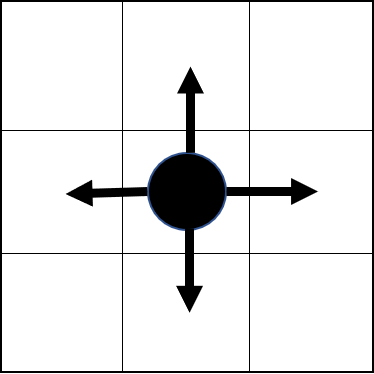
\includegraphics[scale=0.5]{move-direction.png}
\centering\captionsetup{font=small, labelfont=bf}\caption{Moving Derection of an Individual}
}
\parbox[b]{.5\textwidth}{
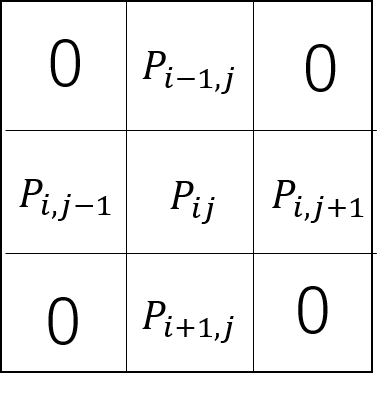
\includegraphics[scale=0.5]{move-possibility.png}
\centering\captionsetup{font=small, labelfont=bf}\caption{Moving Possibility of an Individual}
}
\end{figure}
The Static Floor Field $S_{ij}$ in Equation \eqref{basic} depends on the shortest distance to nearest exit of the cell $(i,j)$. This distance will not change with time going by and will not be affected by other pedestrians. $S_{ij}$ can show effect of geometric layout on evacuation and diverse levels of attraction of different positions in the area. For example, in the process of evacuation, we assume that emergency exit has the highest level of Static Floor Field. 

The Dynamic Floor Field $D_{ij}$ represents the virtual trajectory left behind after an individual's movement. When an individual move one step from a cell $(i,j)$, one boson will be left in this cell, namely $D_{ij}=D_{ij}+1$. In each time unit, one boson will disappear with the possibility of $\delta=50\%$ or move to neighboring cell with the possibility of $\sigma=50\%$.

To consider factors including both seeking nearest distance to exits and desire to avoid congestion, we preliminary determine the possibility of an indicvidual tranferring to cell $(i, j)$ as $P_{ij}$

In the Equation \eqref{basic}, N is a normalization factor.$k_{S}$ and$ k_{D}$ are sensitive parameters of Static Floor Field $S_{ij}$ and Dynamic Floor Field $D_{ij}$. $k_{S} $reflects how familiar with the internal structure an individual is. $k_{D} $shows the tendency of an individual following other visitors. $\mu_{ij} $represents whether the neighboring cell $(i, j) $is occupied by other visitors. If so, we set the value of $\mu_{ij}$ as 1. Otherwise, its value is 0. $\xi_{ij}$depends on whether the neighboring cell $(i, j)$ is occupied by obstacles. If so, we set the value of$ \xi{ij}$ is 0. otherwise, its value is 1.




\subsection{Directional Flow FF Model}
It is clear that the greater the $S_{ij}$ and $D_{ij}$, the more attractive cell$ (i, j)$ is, and then the higher the possibility of transferring to cell$ (i, j)$ is. Besides, if the cell$ (i, j)$ is occupied by a visitor or an obstacle, the value of $P_{ij}$ will be $0$. These settings accord to common sense.\\
When deciding the direction an individual moves in, we need to consider stream of people in visual range. Therefore,we introduce the concept Visual Range $O_{ij}^{rX}$ to describe the density of crowd in four directions: up, down, left ,and right. (X represents directions. It can be U for up, D for down, L for left, and R for right.) The exact value of $O_{ij}^{rX}$ is the number of cells occupied by visitors in the quarter circle with $r$ as its radius in the direction $X$. Now we can improve Equation 3 by adding more factors. Take the upward direction as an example.The improved equation is as follows.

\begin{figure}[H]
	\centering
	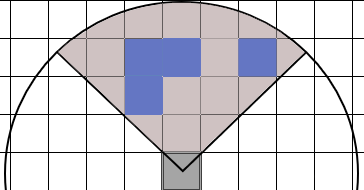
\includegraphics[width=0.3\textwidth]{example-1.png}
      \captionsetup{font=small, labelfont=bf}
	\caption{An example of $O^{rU}_{i,j}=4$}
	\label{calU}
\end{figure}
At each time step, the \textbf{Transition Probability} of the cell $(i, j)$ based on the direction U, D, L, and R are defined as follows:
\begin{equation}
	P^U_{ij}=N_{ij}\cdot exp\left(k_SS_{i-1,j}+k_DD_{i-1,j}+\frac{k_O}{O^{rU}_{i-1,j}}+\frac{k_E}{E^m_{i-1,j}}\right)\left(1-\mu_{i-1,j}\right)\xi_{i-1,j}
	\label{model2}
\end{equation}
In Equation \eqref{model2}, when the parameters $k_O$ and $k_E$ are both given the value of zero, the improved model degenerates to the Floor Field CA model.


\subsection{Directional Visual Field FF Model}
In some certain circumstances, a group of people will gather in an area, which is called heterogeneous distributed \cite{148} . In a museum, take the Louvre Museum for example, people tend to gather around the narrator. When emergency occurs, this group of people will be considered as centralized distributed at the initial time.

In previous researches, visitors are supposed to have the full knowledge of the situation around, the location of the exit door, the layout of the obstacles, and some other important factors. However, few researches cast light on the fact that the vision of the visitors is limited. The evacuation of the vision-limited visitors must also be considered. \cite{70}

The \textbf{directional visual field} of a cell is defined as the number of cells that are not occupied by a visitor in each direction. In this section, every cell has four directional visual field. The directional visual field of cell $(i,j)$ is labeled as $V^{rU}_{ij}$, $V^{rD}_{ij}$, $V^{rL}_{ij}$, and $V^{rR}_{ij}$. $V^{rU}_{ij}$ is the number of the empty cell in the U direction. 

At each time step, the transition probability of the cell $(i,j)$ in direction U is defined as follows:
\begin{equation}
	P^U_{ij}=N_{ij}\cdot exp\left[k_SS_{i-1,j}+k_DD_{i-1,j}+k_VV^{U}_{i-1.j}+\sum_{m\in U}\left(k_CC^m_l+\frac{k_E}{E^m_{i-1,j}}\right)\right]\left(1-\mu_{i-1,j}\right)\xi_{i-1,j}
	\label{final}
\end{equation}

In equation \eqref{final}, $N_{ij}$ is the standardization factor to ensure that $P^U_{ij}+P^D_{ij}+P^L_{ij}+P^R_{ij}=1$. $k_V$ is a parameter that indicates the sensitivity of the viusal field of a certain directional. $C^m_l$ signifies the \textbf{efficacious spare capacity} of the entrance $m$. It is defined as the number of the empty cell in the efficacious space around the entrance $m$. The efficacious space does not need to meet any requirements. For the sake of convenience, we define the efficacious space to be a $1/2$ circle with a radius of $l$, as is shown in the Figure \ref{calV}. Apparently, if the visitors accumulate at the entrance, the efficacious space of the entrance will shrink. $k_C$ is used to indicate the sensitivity of the variable $C^m_l$. 
\begin{figure}[H]
	\centering
	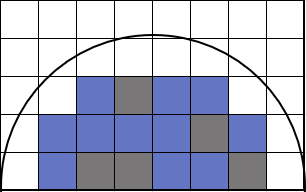
\includegraphics[width=0.3\textwidth]{example-half.png}
\captionsetup{font=small, labelfont=bf}
	\caption{The Definition of the Spare Capacity $C^m_l$. In this figure, $l=4$. The efficacious space of contains $16$ complete cells. The grey cells indicate that the cell is empty, so $C^4_m=11$. }
	\label{calV}
\end{figure}

In Equation \eqref{final}, if the parameters $k_O$, $k_E$, and $k_V$ all take the value of zero, the improved model will automatically degenerates to the origin CA model.

\subsection{Remainder Directional Visual Field}
By considering the directional visual field, visitors can choose the target cell more reasonably, which will help them to make good use of all the four main entrances in the Louvre Museum. In reality, visitors not only evaluate the situation in front of them, but also considere the flow of people in the other three directions. In order to describe their forecast of the flow of the people in the other three directions, we introduce the concept of the \textbf{Remainder Directional Visual Field CA Model}.

in the Directional Visual Field Model, the directional vision field $V^r_{ij}$ is used to identify the visitors' forecast in the visual field. In Figure \ref{calRV}, the grey area ($1/4$ circle) on the center cell's upper side is its visual field. We define the other $3/4$ circle as the \textbf{Remainder Directional Visual Field}. The number of the empty cells in the remainder direction visual field is defined as $RV^{rU}_{ij}$. Similarly, we can define $RV^{rD}_{ij}$, $RV^{rL}_{ij}$, and $RV^{rR}_{ij}$ based on the other three directions. If $RV^{rU}_{ij}$ is rather large, the visitor will definitely choose to go to the cell adjacent to the current cell in the U direction. 

\begin{figure}[H]
	\centering
	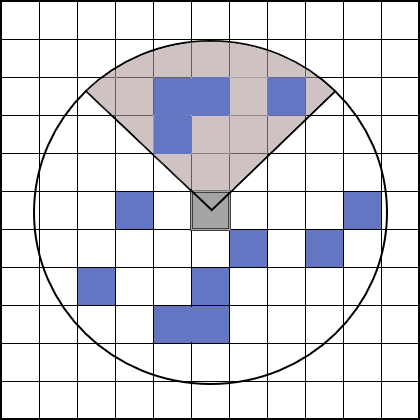
\includegraphics[width=0.3\textwidth]{example.png}
\captionsetup{font=small, labelfont=bf}
	\caption{The Definition of the Remainder Direction Visual Field $RV^{rU}_{ij}$. In this figure, the number of the cells in the remainder direction visual field that are occupied (blue) is 8, so $RV^{rU}_{ij}=8$}
	\label{calRV}
\end{figure}

In each time step, the visitor that occupys the cell have 4 choices to move to an unoccupied cell adjacent. The probability is given by Equation \ref{eqRV}. $k_{RV}$ is a parameter to signify the sensitivity of the variable $RV^{rU}_{i-1,j}$

\begin{dmath}
	P^U_{ij}=N_{ij}\cdot exp\left[k_SS_{i-1,j}+k_DD_{i-1,j}+k_VV^{U}_{i-1.j}+k_{RV}RV^{rU}_{i-1,j}+\sum_{m\in U}\left(k_CC^m_l+\frac{k_E}{E^m_{i-1,j}}\right)\right] \\  \left(1-\mu_{i-1,j}\right)\xi_{i-1,j}.
	\label{eqRV}
\end{dmath}

\section{Simulation of Extended FF Model}
\subsection{Evacuation Scene and Parameter Setting}
In our model, visitors are average distributed by insertting the density value. Then by loading the map, we can get the evacuation scene.The parameters are set as:
$$
k_D = 1.0, k_S = 2.0, k_E = 2, k_C = 0.1, k_V = 0.5, k_{RV} = 0.5 
$$

\subsection{Evacuation Space-Time Figure}
We load the data of stairs, exits, $S_{ij}$ and floor files and run the remedy.py program, then we get the simulation of our evacuation model.\\
The Space-Time Figure for Floor 1 is shown below:
\begin{figure}[H]
\parbox[b]{.5\textwidth}{
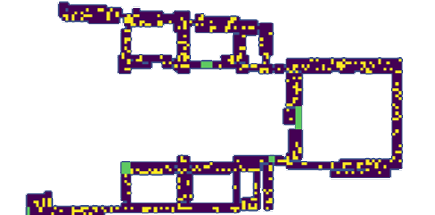
\includegraphics[scale=0.7]{1-1}
\centering\captionsetup{font=small, labelfont=bf}\caption{Floor1 S-T Figure after time 0}
}
\parbox[b]{.5\textwidth}{
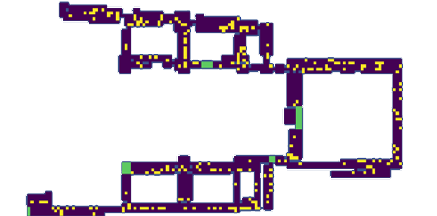
\includegraphics[scale=0.7]{1-2}
\centering\captionsetup{font=small, labelfont=bf}\caption{Floor1 S-T Figure after time 750}
}
\parbox[b]{.5\textwidth}{
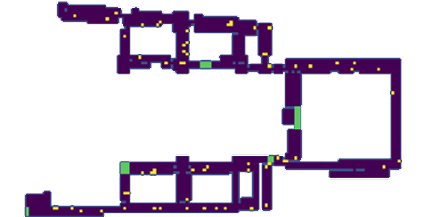
\includegraphics[scale=0.7]{1-3}
\centering\captionsetup{font=small, labelfont=bf}\caption{Floor1 S-T Figure after time 500}
}
\parbox[b]{.5\textwidth}{
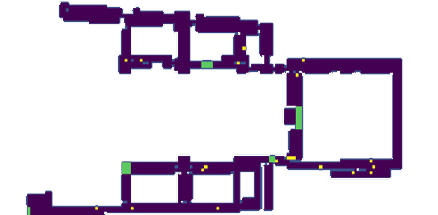
\includegraphics[scale=0.7]{1-4}
\centering\captionsetup{font=small, labelfont=bf}\caption{Floor1 S-T Figure after time 750}
}
\end{figure}

The Space Time Figure for the other three floors are shown in Appendix.

    \subsection{Sensitivity Analysis of Parameters}
We probe into the sensitivity of some parameters in our Extended Floor Field models, As shown in Figure \ref{v-s}. Generally speaking, when we change $k_S$ from $1$ to $2.5$, the total time steps that the visitors need to escape decrease. When we increase $k_V$ from $0.05$ to $0.25$, the total time steps reach it minimum when $k_V=0.1$. This indicates that set the value of $k_V$ to 0.1 can be the most effictive plan in case of the Louvre Museum. Moreover, Figure \ref{v-d} shows the variation when we change $k_D$ from 0 to 3. As we can see, with $k_D$ increasing, the total time steps increase dramatically. When we increase $k_V$ from $0.05$ to $0.3$, the total time steps reach it minimum when $k_V=$ is between 0.1 and 0.15.

\begin{figure}[H]
	\parbox[b]{.5\textwidth}{
		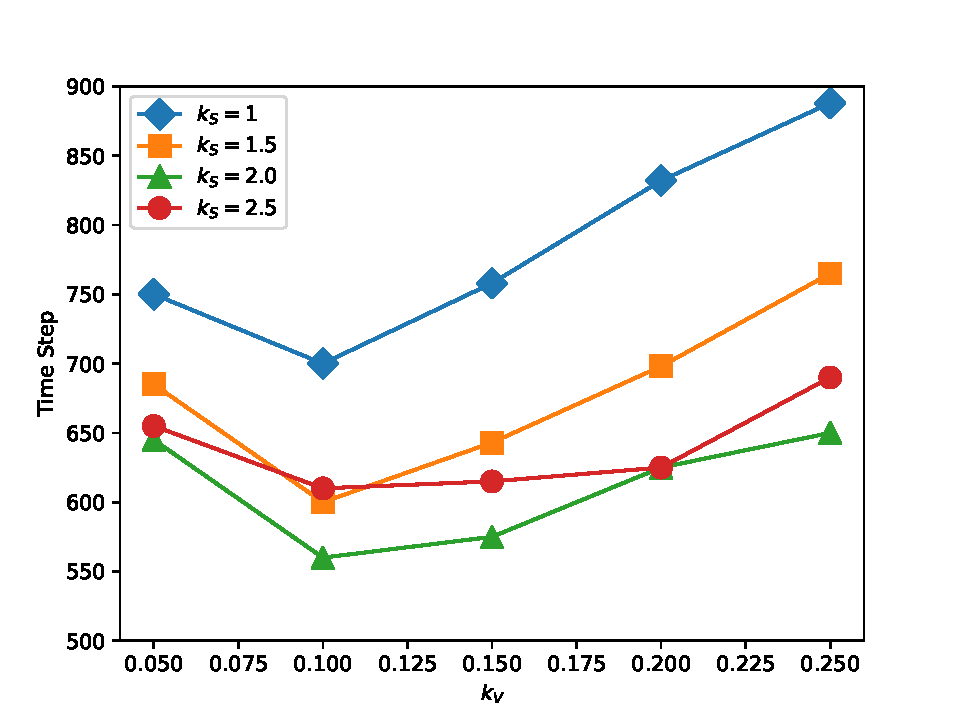
\includegraphics[scale=0.5]{Time-kv-ks.pdf}
		\centering
		\captionsetup{font=small, labelfont=bf}
		\caption{Relation Between $T$ and $k_V$ When  \\$k_D=1,\ k_C=0.1,\ and\ k_E=2$}
		\label{v-s}
	}
	\parbox[b]{.5\textwidth}{
		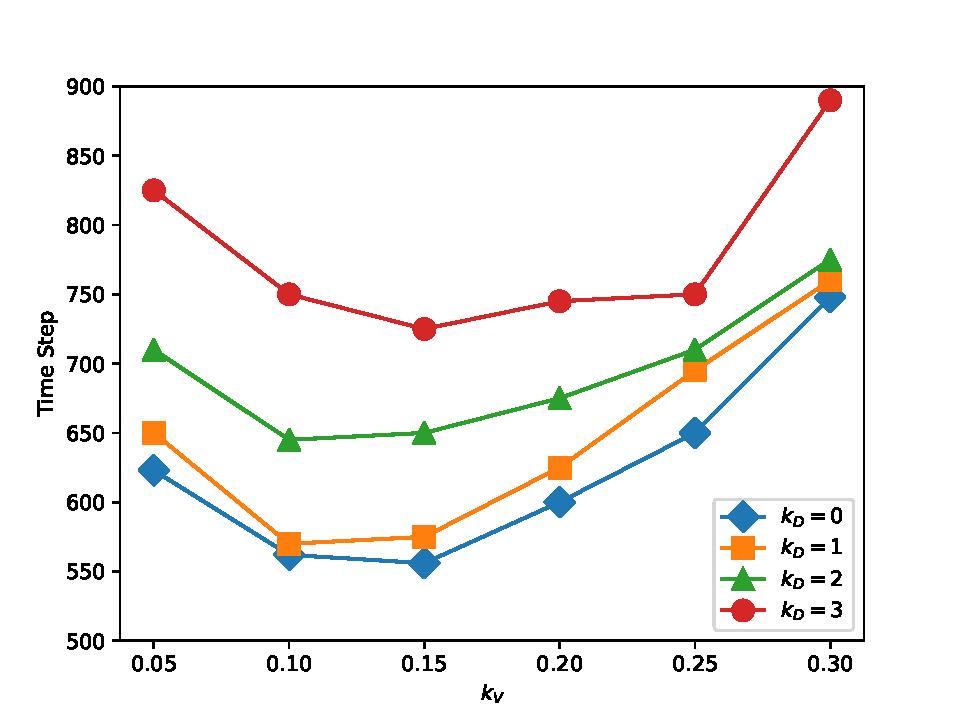
\includegraphics[scale=0.5]{Time-kv-kd.pdf}
		\centering
		\captionsetup{font=small, labelfont=bf}
		\caption{Relation Between $T$ and $k_V$ When \\ $k_D=2,\ k_C=0.1,\ and\ k_E=2$}
		\label{v-d}
	}
\end{figure}

Figure \ref{tr} shows the relationship between the average evacuation time $T$ and the radius $r$ of the influenced area. When $r\in\left[2,\ 3\right]$, $T$ increases and decreases when $r$ increases. $T$ reaches its maximun when $r=3$.
\begin{figure}[H]
    \centering
    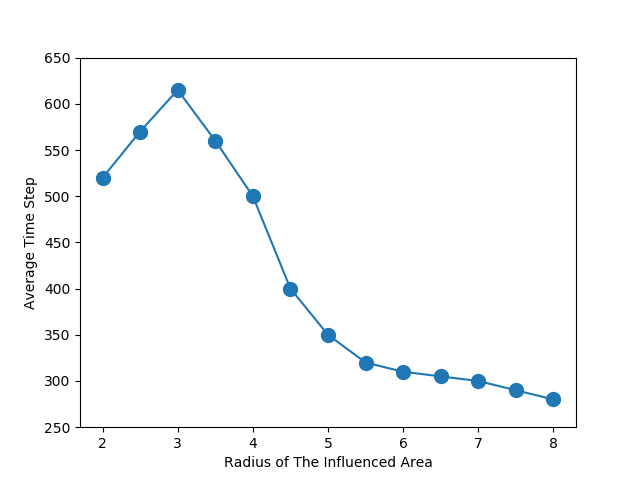
\includegraphics[width=0.45\textwidth]{T-r.png}
    \caption{Relation Between $T$ and r}
    \label{tr}
\end{figure}


    \subsection{Simulation of Various Emergencies}
    The impact of emergencies on evacuation can be categorized into two classes: static emergencies such as terrorist attack and
    landslide, and dynamic emergencies like fire.

    For static emergencies, we only need to calculated the affected area and change the map settings, and the Remainder Directional Visual Field CA Model still applies. For examle, if a rectangular area with coordination from (a,b) to (c,d) on floor1 was affected, we only need to change the value of corresponding coordination of matrix stored in floor1.npy file into 1. 

    For dynamic emergencies, we take fire as example.The fire repulsion force $F_{ij}$ is determined according to the location from the fire occurance area and the fire spreading situation. Generally speaking, in each time step, the most dangerous area(cell point) is determined first according to the spread of fire, and then the fire repulsion force of other cells is calculated accordingly. The closer people is to the most dangerous cell, the greater the value of $F_{ij}$ is. For determination of the most dangerous area, the fire spread model is used, which considers that the fire develpment conforms to a certain process of diffusion and attenuation, which is shown in Equation \eqref{fire} :
    \begin{equation}
        \frac{\partial E}{\partial t} = \alpha \Delta E - \beta E
    \label{fire}    
    \end{equation} 

    E is the degree to which the cell considered is affected by fire, $\alpha$ is the diffusion coefficient, and $\beta$ is the attenuation coefficient. $\Delta E$ is the difference between the degree of fire influence of considered cell and surrounding cell.

\subsection{Individual Heterogeneity of a Population}
\subsubsection{Gender Differences}
 We grasp information from the website of Louvre that $48\%$visitors are male and $52\%$are female. \cite{gender1} The proportion is relatively equal. In the early 1960s, Henderson etc. \cite{gender2}has researched on the population anisotropy caused by sexual difference. They first observed large-scale crowd movement and conduct a census on the distribution of moving speed of more than 2,000 people of different sexes and ages. The statistics show that there exists huge difference on speed distribution between men and women. Besides, women are more likely to feel insecure. Bryan etc. \cite{gender3} researched on the first reaction of Americans when fire broke out. The results show that the percentage of men whose first reaction is “looking for the source of fire” and “grasping fire extinguisher” are higher than that of women, while the percentage of women whose first reaction is “notifying the fire department”and “helping families escape” is higher than that of men. Zhao etc. \cite{gender4} researched on a fire happened in a high-rise building. The statistics show great diversity in first reaction and pre-action time. When fire occurs, women more tend to escape immediately. Consequently, the pre-action time of women is much lower than that of men. Now we can conclude that for evacuation sexual difference is a significant factor.

In the normal evacuation process, the CA model updates the state of every individuals at the same time. That is to say, in each time step, we need to decide next position of every individuals according to the set rule. Now we need to solve the problem how to handle the situation where several individuals choose the same cell. There may be 4 individuals competing for one cell in the same time unit. For each individual, there is a large number of ways to win in the competition, so it is difficult to calculate the winning possibility of each individual and then decide the winner. We take the following measure to decide the winner.
\begin{tabbing}
\textbf{For}\=(\=each \=cell)\\
\>\{\\
\>\> Statistics the number of individuals who move into this cell in the time unit;\\
\>\>Judge the gender of every individuals;\\
\>\>\textbf{if}(\= individuals entering this cell are all male or female)\\
\>\>\>\textbf{then} randomly select one at equal possibility;\\
\>\>\textbf{else if}(individuals entering this cell including both male and female)\\
\>\>\>\textbf{then} two-two competition takes place between everyone who enter this cell;\\
\>\>\{\\
\>\>\textbf{if}(of the opposite sex)\\
\>\>\>The winning possibility of a woman is $P_{c}$ and failed one will be eliminated;\\
\>\>\textbf{if}(of the same sex)\\
\>\>\>Choose winner from the two at an equal possibility and failed one will be eliminated;\\
\>\>\}\\
\>\>return the remaining unselected ones to their original place;\\
\>\}\\
\end{tabbing}
Above all, we pay attention to the changing rule of average evacuation time of male and female when $P_{c}$ differs. We can see from the Figure\ref{gender} that when $P_c=0.5$, the number of women at the exits approximately equals that of men. However, when $P_c=0.2$, there is more women in the exits than men. This agrees with the phenomenon we observe in real life: women are marginalized of first transcend and then fall behind.
Consequently, we set gender as an characteristic of an individual in our model. When several individuals decide to move to the same cell, we decide their possibility of winning on gender.
According to our simulation results, the winning possibility of one man is $0.8$ while that of one woman is $ 0.2$. 
\begin{figure}[H]
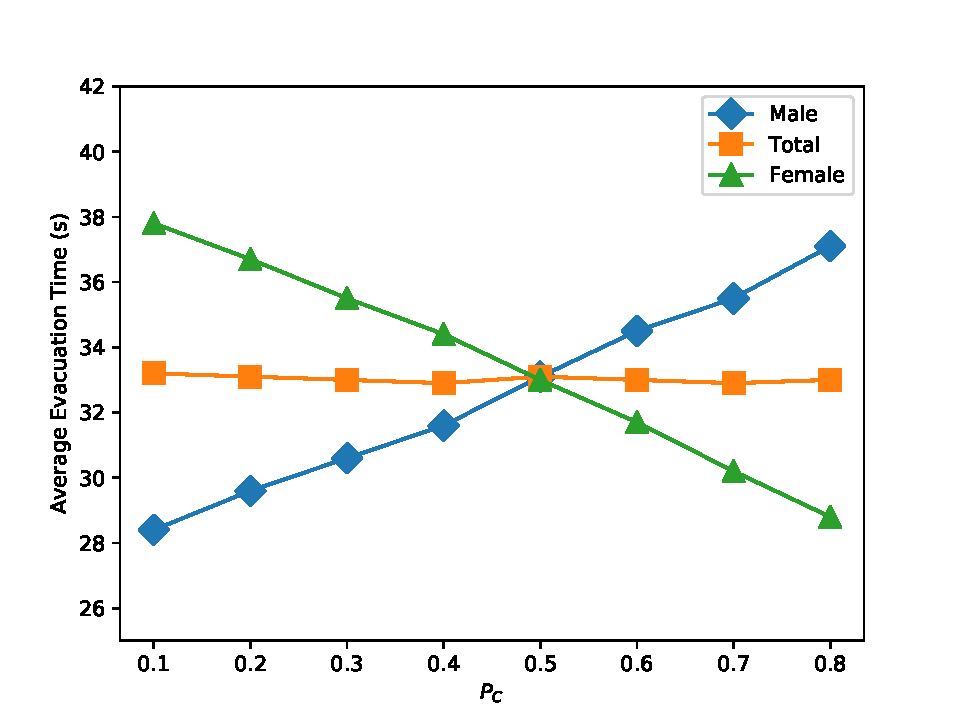
\includegraphics[scale=0.5]{gender}
\centering\captionsetup{font=small, labelfont=bf}\caption{Average Evacuation Time of Male and Female with $P_c$ changing}\label{gender}
\end{figure}
\subsubsection{Identity Differences}
Different people usually have different characteristics. We show this by adding more factors into an individual in our model. There are both able-bodied and disable individuals. We introduce this characteristic into our model by adjusting the moving speed of individuals. 
We learn from an investigation of  American Centers for Disease Control and Prevention \cite{disabled}that there is about $22\%$ people in American are disabled. To simplify our model, we select the disabled ones from all visitors at an possibility of $20\%$. For disabled ones, we set their moving speed as $0.5$ miles per hour while for able-bodied ones, their moving speed remains $1$ mile per hour.




\section{Tasks and Actions}
\subsection{Generalization of the Evacuation Model}
Our model is not just limited to applying to Louvre Museum. With basic steps abstract from our model, we can adapt and implement our model for other large and crowded structures. The basic steps of our model to analyse one structure is:
\begin{itemize}
\item Acquiring information about the internal layout of the structure.
\item Looking for or drawing two-dimensional map of each floor of the structure.
\item Processing the map to programmable image by omitting unnecessary information and changing color. 
\item Employing CA Model and A-Star Algorithm to simulate the process of evacuation.
\item Analysing the simulation result of our model and drawing a conclusion. 
\end{itemize}
Our method of processing image applies broadly. We can process any map of a structure through our algorithm. Therefore, we can design evacuation plan for a wide variety of large and crowded structures.	
\subsection{Policy}
We can learn from experiment results that if the visitors can know more about the internal structure of the building including the distribution of exits , the evacuation time will be shortened greatly. 
\begin{itemize}
\item
Since visitors’ unfamiliarity with the distribution of exits will result in waste of time in evacuation. We suggest that the museum leaders inform the visitors of the exits before they enter the museum. The practical measures can be marking the exits on tourist maps strikingly, adding reminders of exits to audio tour guide, or directly telling visitors both the position of exits and the importance of knowing exits for evacuation. Moreover, posting signs to direct the escape trunk also helps.
\item 
To increase the safety and efficiency of the process of evacuation, we advise that museum leaders arrange staff to guide direction and maintain order especially in the bottleneck so that visitors can leave the building through the most appropriate exit and serious congestion will not happen. Additionally, we recommend that the museum should have emergency dills frequently to ensure that staff know how to handle the situation in face of emergency.
\item 
We suggest the leaders of museum making full use of technology. For example, we can take advantage of the existing online application “Affluences” by adding the function that showing how crowded an exit is to the APP. In this way, visitors can make decision on exit choosing with adequate information.
\item
We advise the museum leaders that under the circumstances of emergency, we need to take noticeable measures to inform the visitors of the position of exits. We recommend to equip the museum with display screen and audio alarm system. When emergency happens, the staff of museum can guide evacuation by showing escape route on the screen and prompting how to have a quick access to exits through the audio alarm.
\item
We advice the leaders to set limits on the reception number of tourists. Otherwise, too many visitors in the museum may lead to long evacuation time, which is a potential risk.
\item
For foreign visitors, language barrier may prevent them from evacuating in time. We advise museum leaders to pay special attention to foreigners. For example, we can add evacuation alarm to the audio tour guide for foreign visitors. Moreover, we can make evacuation signs in various languages.
\end{itemize}

\section{Strengths and Weaknesses}
\subsection{Strengths}
\begin{enumerate}
	\item Our model uses the Grayscale Denoisie Method to transfer a flat 2D floor map to a matrix, which can roughly represent all the necessary details of the floor. This feature greatly adds to the flexibility of our Extended Model, so it can be used to handle various buildings except Louvre Museum.
	\item The calculation of the shortest route is based on heuristic algorithm and pre-stored on local computer before doing simulation, which saves much time.
	\item our Extended Floor Field Model is based on the Celluar Automata Model, which is simple and convenient. What's more, Extended Floor Field Model can focus on the whole picture without worring about the details.
	\item Out models are derived step by step, so the final model is rather trustworthy.
\end{enumerate}
\subsection{Weaknesses}
\begin{enumerate}
	\item We neglect some factors such as the exit points of the Louvre Museum because we lack the accurate position data of those points, which may result in errors in some certain circumstances. 
	\item The data we derived from the Grayscale Denoisie Method is too large and is not suitable for our calculation, so we make some simplification, which may lead to the derivation of the final result.
	\item In Sensitivity Analysis Section, the parameters are not analysized due to their numbers, which means the paramaters setting may not be the optimum solution. 
\end{enumerate}


\section{Conclusions}
In this paper, we first derive a simple map of the Louvre Museum by grayscale denoise method. Then we apply the hierarchical A* algorithm to calculate the shortest path between any given point and the four main entrances in the Louvre Museum. At last we implement a Extended Floor Field evacuation model, which is based on the cellular automata model, to simulate the process of the realtime emergency escape. Based on the result of the Extended FF model, we propose a series of concrete actions for the Louvre Museum to meet the targets. Finally, we conduct sensitivity analysis of some parameters in our model and discuss the strengths and weakness of our work.
\addcontentsline{toc}{section}{References}
\bibliographystyle{unsrt}
\bibliography{reference}



\newpage
\noindent\textbf{\LARGE{Appendix}}

\small

\noindent\textbf{\Large{Space_Time Figure for Floor2, Floor1, Floo1-1:}}\\

\noindent\textbf{The Space-Time Figure for Floor 2 is shown below:}
\begin{figure}[ht]
\parbox[b]{.5\textwidth}{
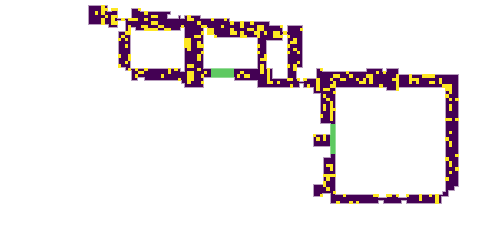
\includegraphics[scale=0.7]{2-1}
\centering\captionsetup{font=small, labelfont=bf}\caption{Floor2 S-T Figure after time 0}
}
\parbox[b]{.5\textwidth}{
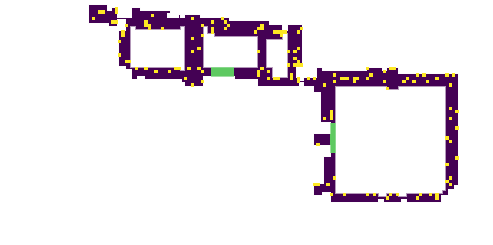
\includegraphics[scale=0.7]{2-2}
\centering\captionsetup{font=small, labelfont=bf}\caption{Floor2 S-T Figure after time 250}
}
\parbox[b]{.5\textwidth}{
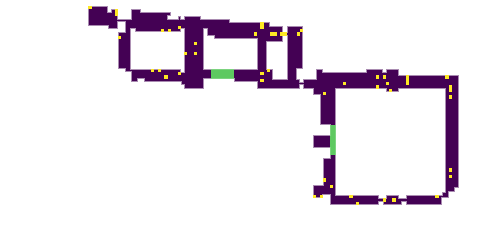
\includegraphics[scale=0.7]{2-3}
\centering\captionsetup{font=small, labelfont=bf}\caption{Floor2 S-T Figure after time 500}
}
\parbox[b]{.5\textwidth}{
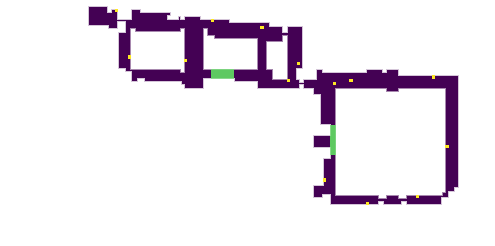
\includegraphics[scale=0.7]{2-4}
\centering\captionsetup{font=small, labelfont=bf}\caption{Floor2 S-T Figure after time 750}
}
\end{figure}

\noindent\textbf{The Space-Time Figure for Floor 0 is shown below:}
\begin{figure}[ht]
\parbox[b]{.5\textwidth}{
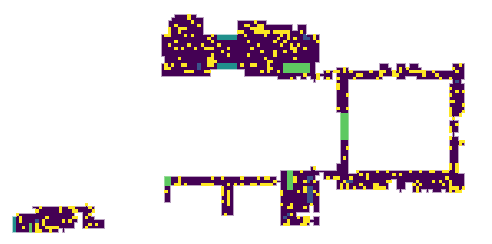
\includegraphics[scale=0.7]{0-1}
\centering\captionsetup{font=small, labelfont=bf}\caption{Floor0 S-T Figure after time 0}
}
\parbox[b]{.5\textwidth}{
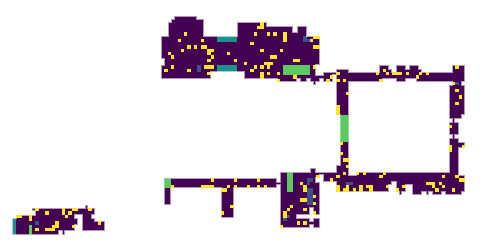
\includegraphics[scale=0.7]{0-2}
\centering\captionsetup{font=small, labelfont=bf}\caption{Floor0 S-T Figure after time 250}
}
\parbox[b]{.5\textwidth}{
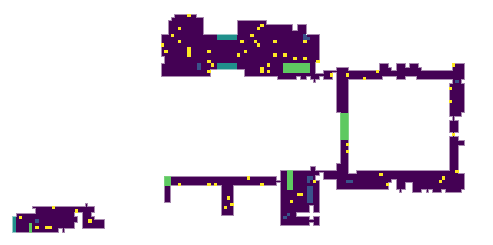
\includegraphics[scale=0.7]{0-3}
\centering\captionsetup{font=small, labelfont=bf}\caption{Floor0 S-T Figure after time 500}
}
\parbox[b]{.5\textwidth}{
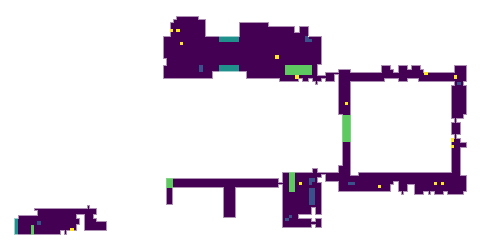
\includegraphics[scale=0.7]{0-4}
\centering\captionsetup{font=small, labelfont=bf}\caption{Floor0 S-T Figure after time 750}
}
\end{figure}

\newpage
\noindent\textbf{The Space-Time Figure for Floor-1 is shown below:}
\begin{figure}[H]
\parbox[b]{.5\textwidth}{
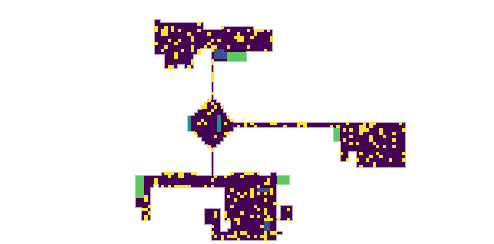
\includegraphics[scale=0.7]{-1-1}
\centering\captionsetup{font=small, labelfont=bf}\caption{Floor-1 S-T Figure after time 0}
}
\parbox[b]{.5\textwidth}{
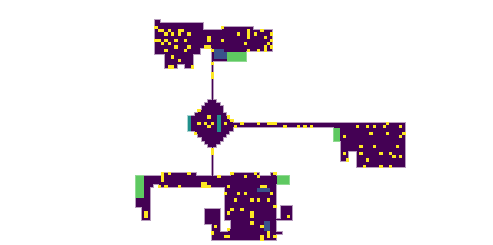
\includegraphics[scale=0.7]{-1-2}
\centering\captionsetup{font=small, labelfont=bf}\caption{Floor-1 S-T Figure after time 250}
}
\parbox[b]{.5\textwidth}{
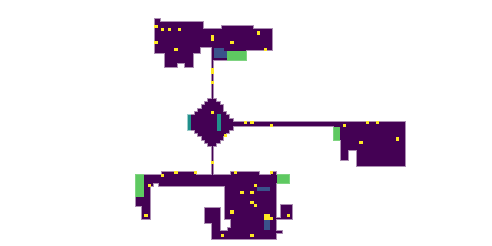
\includegraphics[scale=0.7]{-1-3}
\centering\captionsetup{font=small, labelfont=bf}\caption{Floor-1 S-T Figure after time 500}
}
\parbox[b]{.5\textwidth}{
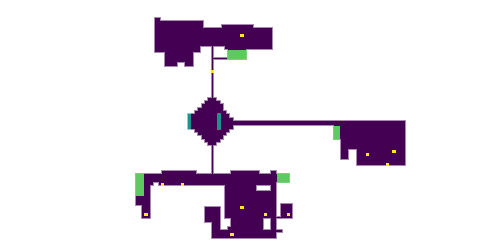
\includegraphics[scale=0.7]{-1-4}
\centering\captionsetup{font=small, labelfont=bf}\caption{Floor-1 S-T Figure after time 750}
}
\end{figure}

\noindent\textbf{\Large{Python Program for Grayscale Process of the Maps}}
\lstset{
basicstyle=\sffamily,
keywordstyle=\bfseries,
commentstyle=\rmfamily\itshape,
stringstyle=\ttfamily,
flexiblecolumns,
numbers=left,
numberstyle=\footnotesize}
\begin{lstlisting}[language=Python]
# import sys,os
from PIL import Image
import numpy as np

image = Image.open("floor-1_proto.png")  
image = image.convert("RGB")
print(image.format)  
print(image.size)  
print(image.mode)  
data = image.getdata()
data = np.matrix(data)
print(data.shape)

width = image.size[0]
height = image.size[1]
for i in range(0, width):
    for j in range(0, height):
        data = (image.getpixel((i, j)))
        # if not ((data[0] == 200 and data[1] == 202 and data[2] == 203)
        #         or (data[0] == 122 and data[1] == 122 and data[2] == 122)):
        #     image.putpixel((i, j), (255, 255, 255))
        if (data[0] == 200 and data[1] == 202 and data[2] == 203)
            or (data[0] == 200 and data[1] == 202 and data[2] == 203):
            image.putpixel((i, j), (0, 0, 0))
        elif data[0] == 122 and data[1] == 122 and data[2] == 122:
            image.putpixel((i, j), (0, 0, 0))
        else:
            image.putpixel((i, j), (255, 255, 255))
image.show()
image.save('D:/jinh/desktop/matrix/floor-1_pixel.BMP')
\end{lstlisting}


\noindent\textbf{\Large{Python Program for Graph-to-Matrix Process}}
\lstset{
basicstyle=\sffamily,
keywordstyle=\bfseries,
commentstyle=\rmfamily\itshape,
stringstyle=\ttfamily,
flexiblecolumns,
numbers=left,
numberstyle=\footnotesize}
\begin{lstlisting}[language=Python]
    from PIL import Image
    import numpy as np
    
    
    # image = Image.open('./matrix/floor/floor-1.png') 
    image = Image.open('./floor_new/floorm1.png')
    print(image.format)  
    print(image.size)  
    print(image.mode)  
    
    length = image.size[0]
    width = image.size[1]
    
    data = image.getdata()
    data = np.matrix(data)
    print(data.shape)
    
    sel = data[:, 0]
    
    data = np.reshape(sel, (length, width))
    output = np.zeros((length, width))
    ite1 = 0
    ite2 = 0
    x = 0
    for i in range(length):
        for j in range(width):
            if 134 > data[i, j] >= 0: #Black 空地
                output[i, j] = 0
                ite1 = ite1 + 1
            elif 200 < data[i, j] <= 255: #White 墙壁
                output[i, j] = 1
                ite2 = ite2 + 1
            elif data[i, j] == 134: #gray134 楼梯
                output[i, j] = 2
            elif data[i, j] == 200: #不知道颜色 门
                output[i, j] = 3
            else: 
                output[i, j] = 1
    
    print(ite1)
    print(ite2)
    
    output = np.reshape(output, (width, length))
    print(output.shape)
    
    
    # np.save('./floor_data/floor-1.npy', output)
    np.save('./floor_data_new/floorm1.npy', output)
    np.savetxt('./floor_data_new/floorm1.csv', output, delimiter=',')
    
\end{lstlisting}


\noindent\textbf{\Large{Python Program for Map De-noising}}
\lstset{
basicstyle=\sffamily,
keywordstyle=\bfseries,
commentstyle=\rmfamily\itshape,
stringstyle=\ttfamily,
flexiblecolumns,
numbers=left,
numberstyle=\footnotesize}
\begin{lstlisting}[language=Python]
# encoding: utf-8

import numpy as np
from PIL import Image
import matplotlib.pyplot as plt
import math
import random
import cv2
import scipy.misc
import scipy.signal
import scipy.ndimage


def medium_filter(im, x, y, step):
    sum_s = []
    for k in range(-int(step / 2), int(step / 2) + 1):
        for m in range(-int(step / 2), int(step / 2) + 1):
            sum_s.append(im[x + k][y + m])
    sum_s.sort()
    return sum_s[(int(step * step / 2) + 1)]


def mean_filter(im, x, y, step):
    sum_s = 0
    for k in range(-int(step / 2), int(step / 2) + 1):
        for m in range(-int(step / 2), int(step / 2) + 1):
            sum_s += im[x + k][y + m] / (step * step)
    return sum_s


def convert_2d(r):
    n = 3
    # 3*3 wave filter, each coefficient is 1/9
    window = np.ones((n, n)) / n ** 2
    # using wave filter for image convolution
    # mode = same : showing output size equals input size
    # boundary: representing that we use symmetrical boundary conditions to process image edges
    s = scipy.signal.convolve2d(r, window, mode='same', boundary='symm')
    return s.astype(np.uint8)


def add_salt_noise(img):
    rows, cols, dims = img.shape
    R = np.mat(img[:, :, 0])
    G = np.mat(img[:, :, 1])
    B = np.mat(img[:, :, 2])

    Grey_sp = R * 0.299 + G * 0.587 + B * 0.114
    Grey_gs = R * 0.299 + G * 0.587 + B * 0.114

    snr = 0.9
    mu = 0
    sigma = 0.12

    noise_num = int((1 - snr) * rows * cols)

    for i in range(noise_num):
        rand_x = random.randint(0, rows - 1)
        rand_y = random.randint(0, cols - 1)
        if random.randint(0, 1) == 0:
            Grey_sp[rand_x, rand_y] = 0
        else:
            Grey_sp[rand_x, rand_y] = 255

    Grey_gs = Grey_gs + np.random.normal(0, 48, Grey_gs.shape)
    Grey_gs = Grey_gs - np.full(Grey_gs.shape, np.min(Grey_gs))
    Grey_gs = Grey_gs * 255 / np.max(Grey_gs)
    Grey_gs = Grey_gs.astype(np.uint8)

    # Median Filtering
    Grey_sp_mf = scipy.ndimage.median_filter(Grey_sp, (8, 8))
    Grey_gs_mf = scipy.ndimage.median_filter(Grey_gs, (8, 8))

    # Mean Filtering
    n = 3
    window = np.ones((n, n)) / n ** 2
    Grey_sp_me = convert_2d(Grey_sp)
    Grey_gs_me = convert_2d(Grey_gs)

    # plt.subplot(321)
    # plt.title('Grey salt and pepper noise')
    # plt.imshow(Grey_sp, cmap='gray')
    # plt.subplot(322)
    # plt.title('Grey gauss noise')
    # plt.imshow(Grey_gs, cmap='gray')

    plt.subplot(221)
    ## plt.plot()
    plt.title('Grey salt and pepper noise (medium)')
    plt.imshow(Grey_sp_mf, cmap='gray')
    plt.subplot(222)
    plt.title('Grey gauss noise (medium)')
    plt.imshow(Grey_gs_mf, cmap='gray')

    plt.subplot(223)
    plt.title('Grey salt and pepper noise (mean)')
    plt.imshow(Grey_sp_me, cmap='gray')
    plt.subplot(224)
    plt.title('Grey gauss noise (mean)')
    plt.imshow(Grey_gs_me, cmap='gray')
    plt.show()


def main():
    img = np.array(Image.open('floor0_bw.bmp'))

    add_salt_noise(img)


if __name__ == '__main__':
    main()
\end{lstlisting}


\noindent\textbf{\Large{Python Program of A* Algorithm for Route Optimization}}
\lstset{
basicstyle=\sffamily,
keywordstyle=\bfseries,
commentstyle=\rmfamily\itshape,
stringstyle=\ttfamily,
flexiblecolumns,
numbers=left,
numberstyle=\footnotesize}
\begin{lstlisting}[language=Python]
import numpy as np
# import pandas as pd
from heapq import *

def heuristic(a, b):
    return (b[0] - a[0]) ** 2 + (b[1] - a[1]) ** 2


def astar(array, start, goal):
    # neighbors = [(0, 1), (0, -1), (1, 0), (-1, 0), (1, 1), (1, -1), (-1, 1), (-1, -1)]
    neighbors = [(0, 1), (0, -1), (1, 0), (-1, 0)]
    close_set = set()
    came_from = {}
    gscore = {start: 0}
    fscore = {start: heuristic(start, goal)}
    oheap = []

    heappush(oheap, (fscore[start], start))

    while oheap:

        current = heappop(oheap)[1]

        if current == goal:
            data = []
            while current in came_from:
                data.append(current)
                current = came_from[current]
            return data

        close_set.add(current)
        for i, j in neighbors:
            neighbor = current[0] + i, current[1] + j
            tentative_g_score = gscore[current] + heuristic(current, neighbor)
            if 0 <= neighbor[0] < array.shape[0]:
                if 0 <= neighbor[1] < array.shape[1]:
                    if array[neighbor[0]][neighbor[1]] == 1:
                        continue
                else:
                    # array bound y walls
                    continue
            else:
                # array bound x walls
                continue

            if neighbor in close_set and tentative_g_score >= gscore.get(neighbor, 0):
                continue

            if tentative_g_score < gscore.get(neighbor, 0) or neighbor not in [i[1] for i in oheap]:
                came_from[neighbor] = current
                gscore[neighbor] = tentative_g_score
                fscore[neighbor] = tentative_g_score + heuristic(neighbor, goal)
                heappush(oheap, (fscore[neighbor], neighbor))

    return 'F'


floor0_stair = np.loadtxt('./All_Data/floor0_stair.csv', delimiter=',')
nmap = np.loadtxt('./All_Data/floor0.csv', delimiter = ',')

# change
floor_stair = floor0_stair
floor = 0

m = floor0_stair.shape[0]
print(m)


length = nmap.shape[0]  # 11
width = nmap.shape[1]  # 14
a = 0
l_m = 2

S = np.zeros((length, width))

#floor 2
print('S_current = \n')
for k in np.arange(1, m + 1):
    stair_pos = (int(float((floor_stair[k-1 , 2]))), int(float((floor_stair[k-1, 3]))))
    for i in range(length):
        for j in range(width):
            if nmap[i, j] != 1:
                step = astar(nmap, stair_pos, (i, j))
                S[i, j] = len(step)
            elif nmap[i, j] == 1:
                S[i, j] = -1  # -1 represents for WALL
            # S_max = max(S_max, S[i, j])
        #     print(int(S[i, j]), '\t', end='')
        # print('i = %d is done\n'%i)
    # print('\n')
    np.savetxt("./All_Data/S_current_%d_%d.csv"%(floor,k), S,  delimiter = ',')
    print('S_current_%d%d OVER \n'%(floor, k))
# S_max = S.max()

print('\n')
print('S_{ij} = \n')
for k in np.arange(1, m + 1):
    S = np.loadtxt("./All_Data/S_current_%d_%d.csv"%(floor,k), delimiter = ',')
    S_max = S.max()
    for i in range(length):
        for j in range(width):
            if nmap[i, j] != 1:
                S[i, j] = a * l_m + S_max - S[i, j]
            elif nmap[i, j] == 1:
                S[i, j] = -1  # -1 represents for WALL
    #     print(int(S[i, j]), '\t', end='')
    # print('\n')
    np.savetxt("./All_Data/S_ij_%d_%d.csv"%(floor,k), S,  delimiter = ',')
    print('S_ij_%d%d OVER \n'%(floor,k))
\end{lstlisting}






\noindent\textbf{\Large{Python Program for Evacuation Simulation}}
\lstset{
basicstyle=\sffamily,
keywordstyle=\bfseries,
commentstyle=\rmfamily\itshape,
stringstyle=\ttfamily,
flexiblecolumns,
numbers=left,
numberstyle=\footnotesize}
\begin{lstlisting}[language=Python]  
    import numpy as np
    import matplotlib.pyplot as plt
    
    inf = 999
    rho = 0.5
    length, width = 75, 150
    passage, wall, door, stair, man = 0, 1, 2, 3, 4
    
    
    # floorm1 = np.loadtxt('./All_Data/floorm1.csv', delimiter=',')
    # floor0 = np.loadtxt('./All_Data/floor0.csv', delimiter=',')
    floor1 = np.loadtxt('./All_Data/floor1.csv', delimiter=',')
    # floor2 = np.loadtxt('./All_Data/floor2.csv', delimiter=',')
    # floorm1_stair = np.loadtxt('./All_Data/floorm1_stair.csv', delimiter=',')
    # floor0_stair = np.loadtxt('./All_Data/floor0_stair.csv', delimiter=',')
    floor1_stair = np.loadtxt('./All_Data/floor1_stair.csv', delimiter=',')
    # floor2_stair = np.loadtxt('./All_Data/floor2_stair.csv', delimiter=',')
    
    
    
    stair_pos = [(67,10),(68,10),(69,10),(70,10)]
    
    class GameOfLife(object):
        def __init__(self, cells_shape):
            self.cells = np.zeros(cells_shape) #  0没人 1有人
            self.timer = 0
            self.k1 = 0.1
            self.k2 = 2
            self.N = np.zeros(cells_shape) #kesi 函数
            self.D = np.zeros(cells_shape)  # people following
            self.P = np.zeros(cells_shape)  # choose ways
            self.S = np.loadtxt('S{ij}.csv', delimiter=',')  # distance
            self.floor = floor1
            self.d = -1
    
            for i in range(cells_shape[0]):
                for j in range(cells_shape[1]):
                    if self.floor[i][j] == 0:
                        self.cells[i][j] = 1 if np.random.randint(100 + 100 * rho) / 100 > 1 else 0
    
        def update_state(self):
            # buf = np.zeros(self.cells.shape)
            cells = self.cells
            self.D = self.D / 2
    
    
            for i in range(cells.shape[0]):
                for j in range(cells.shape[1]):
                    self.P[i][j] = 0
                    if self.floor[i][j] == passage:
                        #todo 概率公式
                        self.P[i][j] = (self.k1 * self.S[i][j]) * (1 - cells[i][j]) * (1- self.N[i][j])
                        # self.P[i][j] = np.exp(self.k1 * self.S[i][j] + self.k2 * self.D[i][j])
                    elif self.floor[i][j] == door:
                        self.P[i][j] = inf
                    elif self.floor[i][j] == stair:
                        self.P[i][j] = inf
    
            for i in range(cells.shape[0]):
                for j in range(cells.shape[1]):
                    if self.cells[i][j] == 1:
                        direction = -1
                        maxP = 0
                        P_u, P_r, P_l, P_d = 0, 0, 0, 0
                        #todo 通过四个方向概率 算预运动方向direction
                        if i - 1 >= 0:
                            P_u = self.P[i - 1][j]
                        else:
                            P_u = 0
                        if j + 1 < width:
                            P_r = self.P[i][j + 1]
                        else:
                            P_r = 0
                        if i + 1 < length:
                            P_l = self.P[i + 1][j]
                        else:
                            P_l = 0
                        if j - 1 >= 0:
                            P_d = self.P[i][j - 1]
                        else:
                            P_d = 0
                        arr = np.array([P_u, P_r, P_l, P_d])
                        direction = np.argmax(arr)
    
    
                        # choose here
                        if direction == 0 and self.floor[i - 1][j] == 0:   
                            cells[i - 1][j] = 1
                            cells[i][j] = 0
                            self.floor[i - 1][j] = man
                            self.floor[i][j] = 0
                            self.D[i - 1][j] += 10
                            self.d = 0
                        elif direction == 1 and self.floor[i][j + 1] == 0:
                            cells[i][j + 1] = 1
                            cells[i][j] = 0
                            self.floor[i][j + 1] = man
                            self.floor[i][j] = 0
                            self.D[i][j + 1] += 10
                            self.d = 1
                        elif direction == 2 and self.floor[i + 1][j] == 0:
                            cells[i + 1][j] = 1
                            cells[i][j] = 0
                            self.floor[i + 1][j] = man
                            self.floor[i][j] = 0
                            self.D[i + 1][j] += 10
                            self.d = 2
                        elif direction == 3 and self.floor[i][j - 1] == 0:
                            cells[i][j - 1] = 1
                            cells[i][j] = 0
                            self.floor[i][j - 1] = man
                            self.floor[i][j] = 0
                            self.D[i][j - 1] += 10
                            self.d = 3
                        elif direction == 0 and (self.floor[i - 1][j] == 2 or self.floor[i - 1][j] == 3):  #
                            cells[i - 1][j] = 0
                            cells[i][j] = 0
                            self.floor[i][j] = 0
                            self.D[i - 1][j] += 10
                            self.d = 0
                        elif direction == 1 and (self.floor[i][j + 1] == 2 or self.floor[i][j + 1] == 3):
                            cells[i][j + 1] = 0
                            cells[i][j] = 0
                            self.floor[i][j] = 0
                            self.D[i][j + 1] += 10
                            self.d = 1
                        elif direction == 2 and (self.floor[i + 1][j] == 2 or self.floor[i + 1][j] == 3):
                            cells[i + 1][j] = 0
                            cells[i][j] = 0
                            self.floor[i][j] = 0
                            self.D[i + 1][j] += 10
                            self.d = 2
                        elif direction == 3 and (self.floor[i][j - 1] == 2 or self.floor[i][j - 1] == 3):
                            cells[i][j - 1] = 0
                            cells[i][j] = 0
                            self.floor[i][j] = 0
                            self.D[i][j - 1] += 10
                            self.d = 3
                        else: #不动 direction = -1
                            cells[i][j] = 1
                            self.floor[i][j] = man
                            self.D[i][j] += 10
                            self.d = -1
    
            # clear the man in the door
            for i in stair_pos:
                x = i[0]
                y = i[1]
                cells[x][y] = 0
                self.floor[x][y] = 0
    
            self.timer += 1
            # cells[67][10] = cells[68][10] = cells[69][10] = cells[4][29] = cells[9][29] = 0
            # self.floor[26][1] = self.floor[27][1] = self.floor[28][1] = self.floor[4][29] = self.floor[9][29] = 0
            # # self.cells = buf
            # self.timer += 1
    
    
    
    
        def update_and_plot(self, n_iter):
            plt.ion()
            print(game.cells.shape)
    
            for i in range(game.cells.shape[0]):
                for j in range(game.cells.shape[1]):
                    if self.floor[i][j] == 1:
                        self.N[i][j] == 1
                    else:
                        self.N[i][j] == 0
    
            for _ in range(n_iter):
                plt.title('Iter :{}'.format(self.timer))
                self.update_state()
                plt.imshow(self.floor)
                plt.pause(0.2)
            plt.ioff()
    
    
    if __name__ == '__main__':
        game = GameOfLife(cells_shape=(length, width))
        game.update_and_plot(60)
\end{lstlisting}




\end{document}